\documentclass[final,5p,times,twocolumn]{elsarticle}
% \documentclass[review,5p,times,twocolumn]{elsarticle}  % review: 1.5-spaced + line numbers

\let\today\relax
\journal{Computers and Electrical Engineering}

% Line numbers (review aid; comment \linenumbers below for camera-ready)
\usepackage{lineno}
\modulolinenumbers[5]

\usepackage{hyperref}
\makeatletter
\g@addto@macro{\UrlBreaks}{\UrlOrds}
\makeatother
\renewcommand{\UrlFont}{\ttfamily\scriptsize}

\usepackage{amsmath}
\usepackage{amssymb}
\usepackage{amsthm}
\usepackage{epstopdf}
\usepackage{graphicx}
\DeclareGraphicsExtensions{.pdf,.png,.jpg,.eps}
\graphicspath{{./}{../figures/}{figures/}{../tables/}{tables/}}

\usepackage{multirow}
\usepackage{paralist}
\usepackage{booktabs}
\usepackage{tabularx}
\usepackage{xspace}
\usepackage{pifont}
\usepackage{subcaption}
\usepackage{algorithm}
\usepackage{algpseudocode}   % body uses \State/\Comment (algorithmicx), not the old algorithmic
\usepackage{xcolor}

\usepackage{tikz}
\usetikzlibrary{arrows.meta,positioning,calc,fit,shadows,backgrounds,shapes.geometric,shapes.symbols,shapes.misc,decorations.pathreplacing,decorations.pathmorphing,patterns}
\usepackage{pgfplots}
\pgfplotsset{compat=1.18}
\usepgfplotslibrary{fillbetween}

% acmart accessibility macro used inside the figure files -- no-op under elsarticle
\providecommand{\Description}[1]{}

% ──────────────────────────────────────────────────────────────────
%  Macros
% ──────────────────────────────────────────────────────────────────
\newcommand{\todo}[1]{\textcolor{red}{\bf #1}}
\newcommand{\edit}[1]{\textcolor{blue}{#1}}
\newcommand{\info}[1]{\textcolor{gray}{#1}}
\newcommand{\sstitle}[1]{\smallskip\noindent\textbf{#1.\/}}
\newcommand{\smtitle}[1]{\medskip\noindent\textbf{#1.\/}}
\newcommand{\sititle}[1]{{\it #1:\/}}

\newcommand{\toolname}{\texttt{PhishProof}\xspace}
\newcommand{\limit}[1]{\textbf{L#1}}
\newcommand{\req}[1]{\textbf{R#1}}

% math
\newcommand{\bO}{\mathcal{O}}
\newcommand{\R}{\mathbb{R}}
\newcommand{\E}{\mathbb{E}}
\newcommand{\Prob}{\mathbb{P}}
\newcommand{\Var}{\mathrm{Var}}
\newcommand{\Indic}{\mathbf{1}}
\newcommand{\page}{\ensuremath{x}}              % a page under test
\newcommand{\panel}{\ensuremath{\mathcal{M}}}   % the model panel
\newcommand{\Uschema}{\ensuremath{\mathcal{U}}} % evidence-unit schema
\newcommand{\evset}{\ensuremath{E}}             % cited evidence set
\newcommand{\agr}{\ensuremath{A}}               % evidence-level agreement
\newcommand{\grd}{\ensuremath{G}}               % groundedness
\newcommand{\geascore}{\ensuremath{\mathrm{GEA}}} % the score
\newcommand{\gver}{\ensuremath{g}}              % per-unit grounding verifier
\newcommand{\cons}{\ensuremath{C}}              % consensus set
\newcommand{\thr}{\ensuremath{\tau}}            % abstention threshold

\newcommand{\cmark}{\ding{51}}
\newcommand{\xmark}{\ding{55}}

% Harvey balls for the capability table. A raw \tikz is NOT robust inside a
% \caption{} -- it makes ; : | active and breaks caption parsing (this caused the
% \caption@ydblarg / Emergency-stop error). So we pre-render each ball into a box
% once (filled just after \begin{document}) and place it with a robust \usebox,
% which is safe in captions and table cells alike. Keeps amssymb (no wasysym clash).
\newsavebox{\hbFull}
\newsavebox{\hbHalf}
\newsavebox{\hbOpen}
\DeclareRobustCommand{\CIRC}{\usebox{\hbFull}}
\DeclareRobustCommand{\HCIR}{\usebox{\hbHalf}}
\DeclareRobustCommand{\OCIR}{\usebox{\hbOpen}}

\newtheorem{theorem}{Theorem}
\newtheorem{proposition}{Proposition}
\newtheorem{lemma}{Lemma}
\newtheorem{definition}{Definition}
\newtheorem{assumption}{Assumption}

\def\Snospace~{\S{}}
\renewcommand*\sectionautorefname{\Snospace}
\renewcommand*\subsectionautorefname{\Snospace}
\renewcommand*\subsubsectionautorefname{\Snospace}
\renewcommand*\figureautorefname{Fig.}
\renewcommand*\equationautorefname{Eq.}
\renewcommand*\tableautorefname{Tab.}
\newcommand*\algorithmautorefname{Alg.}
\renewcommand*\theoremautorefname{Thm.}
\providecommand*\propositionautorefname{Prop.}
\providecommand*\assumptionautorefname{Assumption}
\providecommand*\definitionautorefname{Def.}
\providecommand*\lemmaautorefname{Lemma}

\clubpenalty=10000
\widowpenalty=10000
\displaywidowpenalty=10000
\brokenpenalty=10000

\begin{document}

% Pre-render the capability-table Harvey balls (see preamble note) so they can be
% placed with \usebox inside \caption{} without activating ; : | .
\sbox{\hbFull}{\tikz[baseline=-0.4ex]{\fill (0,0) circle (0.5ex);}}
\sbox{\hbHalf}{\tikz[baseline=-0.4ex]{\draw[line width=0.5pt] (0,0) circle (0.5ex); \fill (0,0) -- (0,0.5ex) arc (90:-90:0.5ex) -- cycle;}}
\sbox{\hbOpen}{\tikz[baseline=-0.4ex]{\draw[line width=0.5pt] (0,0) circle (0.5ex);}}

\begin{frontmatter}

\title{Trustworthy and Explainable Agents for Phishing Detection with
Grounded Cross-Model Evidence Agreement}

\author[hust]{Xuan Huong Tran}
\ead{Huong.TX261096M@sis.hust.edu.vn}


\author[griffith]{Trinh Pham}
\ead{trinh.pham@griffithuni.edu.au}

\author[griffith]{Thanh Tam Nguyen}
\ead{t.nguyen19@griffith.edu.au}


\affiliation[hust]{organization={Hanoi University of Science and Technology},
            % city={}, postcode={}, state={},
            country={Vietnam}}


\affiliation[griffith]{organization={Griffith University},
            % city={}, postcode={}, state={},
            country={Australia}}



\begin{abstract}
Phishing defenders need a verdict they can trust and a reason they can check. Large
language models are accurate but score trust at the label, so several models can agree on
the right answer while citing different or fabricated evidence. We propose \toolname{}, a
selective detector that reads trust from grounded cross-model evidence agreement (GEA): a
diverse panel emits typed cues from the page's URL, DOM, screenshot, and logo (certificate
and redirect cues when available), verification tools confirm them against the page, and a
held-out split calibrates GEA to a probability of correctness. \toolname{} acts only on
grounded agreement and otherwise abstains, returning verified cues as an explanation.
On \textsc{PhishSel} ($998$ test pages of feed-sourced phishing paired with legitimate login
pages), \toolname{} attains the best-calibrated trust (ECE $0.015$, statistically
significant) and the highest selective accuracy at $80\%$ coverage ($97.0\%$, significant).
Its area-under-risk--coverage is lowest in point estimate ($2.3$) though not statistically
separated from the strongest baseline; it trades top-end deployable coverage (Cov$_{99}$
$0.25$ vs.\ $0.36$) for sharper calibration in the $50$--$80\%$ deployment band. Under
evidence-targeted attacks, abstention on evaded pages reaches $97.5$--$100\%$ while
single-model confidence stays maximally certain; even a white-box, all-cue
adversary -- cloaking the form action, erasing the brand's textual identity, and
occluding the logo simultaneously -- flips more verdicts but \toolname{} abstains
on every one of them ($100\%$, $n{=}50$). Calibrated trust transfers to
unseen brands, and negative ablations show that learned aggregation, larger text models, and
cheaper cascades do not beat the parameter-free design.

\end{abstract}

\begin{keyword}
Phishing detection \sep Cybersecurity \sep Large language models \sep Multi-agent systems
\sep Explainable AI \sep Selective prediction \sep Grounded evidence agreement
\sep Trustworthy AI
\end{keyword}

\end{frontmatter}

% \linenumbers   % camera-ready: keep commented (review copy may uncomment)

\section{Introduction}
\label{sec:intro}

Phishing remains one of the most prevalent and costly cybersecurity threats, and
automated detectors deployed across web browsers, mail gateways, and enterprise
security pipelines are a primary line of defense. A phishing verdict is also a consequential
act: marking a page as phishing drives a blocklist entry, a browser warning, or a
take-down request that pulls a live service off the web. Large language models have sharply raised the accuracy of
such detectors, reading a page's URL, Document Object Model (DOM), rendered screenshot, and certificate
to decide whether it impersonates a brand it does not own~\cite{tan2024phishllm,
li2024knowphish}. Yet accuracy is only half of what a deployment needs: the
operator who must justify a take-down and the user who sees a warning both need a
\emph{reason} they can check, and the system needs a criterion for \emph{when} a
verdict is trustworthy enough to act on without review. For a decision that can be
contested, the bottleneck is no longer whether the model is usually right, but
whether a particular verdict can be \emph{trusted and explained}.

Existing detectors approach this only indirectly. One line runs a single LLM over
the page and reports a class probability or a verbalized
confidence~\cite{tan2024phishllm}; reliability is then a property of that one
model's calibration~\cite{guo2017calibration}. A second line aggregates several
models or several samples -- self-consistency over one
model~\cite{wang2023selfconsistency}, majority voting over an
ensemble~\cite{ensembleornot2024}, or weighted label agreement in the style of
crowd-sourcing and label-free evaluation~\cite{dawid1979maximum,tci2025} -- and
reads reliability off how often the votes concur. A third, recent line builds
multi-agent detectors whose agents specialize on different signals and whose
rationales are merged into a single explanation~\cite{phishdebate2025,
multiphishguard2025}. Together these families cover much of the space of accuracy
and aggregation.

\begin{figure*}[!h]
\centering
% ---- palette -------------------------------------------------------------
\definecolor{PPInk}{HTML}{243443}
\definecolor{PPBlue}{HTML}{DCEFF7}
\definecolor{PPMint}{HTML}{DCF2D8}
\definecolor{PPCream}{HTML}{FFF2C6}
\definecolor{PPPeach}{HTML}{FCE2D4}
\definecolor{PPLav}{HTML}{E9E6FF}
\definecolor{PPGreen}{HTML}{2F8F5B}
\definecolor{PPRed}{HTML}{B24A4A}
\definecolor{PPGold}{HTML}{D49B22}
% agent-identity hues (kept distinct from the green/amber/red verdict colors)
\definecolor{PPA}{HTML}{2C6FB0}   % A1 text    -- blue
\definecolor{PPB}{HTML}{6E54C8}   % A2 vision  -- violet
\definecolor{PPC}{HTML}{1F8E8B}   % A3 security-- teal
% small inline half-disc used as the "partial" mark (matches the board stamp)
\newcommand{\hpart}{\tikz[baseline=-0.42ex]{\begin{scope}\clip (0,0) circle (0.92mm);
  \fill[PPGold!85!black] (-1mm,-1mm) rectangle (0,1mm);\end{scope}
  \draw[line width=0.25pt, PPGold!85!black] (0,0) circle (0.92mm);}}
\resizebox{\textwidth}{!}{%
\begin{tikzpicture}[
  font=\sffamily\scriptsize,
  >=Latex,
  stage/.style={font=\sffamily\tiny\bfseries, text=PPInk, align=left},
  sbadge/.style={circle, fill=PPInk, text=white, font=\sffamily\tiny\bfseries,
    minimum size=3.4mm, inner sep=0pt},
  card/.style={draw=PPInk!45, line width=0.35pt, rounded corners=2.5pt,
    fill=white, inner sep=3pt, align=center,
    drop shadow={shadow xshift=0.25pt, shadow yshift=-0.25pt, fill=black!9}},
  agent/.style={card, fill=white, text width=26mm, minimum height=11.5mm, align=left},
  board/.style={card, fill=PPMint!22, minimum width=44mm, minimum height=41mm},
  gauge/.style={card, fill=PPLav!26, minimum width=33mm, minimum height=37mm},
  decision/.style={card, text width=34mm, minimum height=19mm, align=left},
  erow/.style={draw=PPInk!22, line width=0.3pt, rounded corners=2pt,
    fill=white, minimum width=40mm, minimum height=9.4mm, inner sep=0pt},
  toolchip/.style={draw=PPInk!28, line width=0.25pt, rounded corners=1pt,
    fill=PPInk!4, inner sep=1.3pt, font=\sffamily\fontsize{4.5}{5}\selectfont, text=PPInk!82},
  flow/.style={-{Latex[length=1.6mm]}, line width=0.55pt, draw=PPInk!72},
  weakflow/.style={-{Latex[length=1.35mm]}, line width=0.5pt, draw=PPRed!75, dashed},
  thin/.style={line width=0.25pt, draw=PPInk!30},
  pin/.style={circle, draw=white, line width=0.2pt, minimum size=2.7mm,
    inner sep=0pt, font=\sffamily\fontsize{4.2}{4.4}\selectfont\bfseries, text=white},
  stamp/.style={circle, line width=0.3pt, minimum size=4mm, inner sep=0pt,
    font=\sffamily\tiny\bfseries},
  % ---------- icon library (drawn, so they scale with the figure) ----------
  pics/ic text/.style={code={
    \draw[line width=0.3pt, rounded corners=0.2mm] (-1mm,-1.3mm) rectangle (1mm,1.3mm);
    \draw[line width=0.28pt] (-0.6mm,0.8mm)--(0.6mm,0.8mm);
    \draw[line width=0.28pt] (-0.6mm,0.3mm)--(0.6mm,0.3mm);
    \draw[line width=0.28pt] (-0.6mm,-0.2mm)--(0.6mm,-0.2mm);
    \draw[line width=0.28pt] (-0.6mm,-0.7mm)--(0.2mm,-0.7mm);}},
  pics/ic eye/.style={code={
    \draw[line width=0.32pt] (-1.25mm,0) .. controls (-0.5mm,1.05mm) and (0.5mm,1.05mm) .. (1.25mm,0)
       .. controls (0.5mm,-1.05mm) and (-0.5mm,-1.05mm) .. (-1.25mm,0) -- cycle;
    \fill (0,0) circle (0.46mm);}},
  pics/ic shield/.style={code={
    \draw[line width=0.32pt, line join=round] (0,1.45mm) -- (1.2mm,0.85mm) -- (1.2mm,-0.35mm)
      .. controls (1.2mm,-1.05mm) and (0.55mm,-1.4mm) .. (0,-1.6mm)
      .. controls (-0.55mm,-1.4mm) and (-1.2mm,-1.05mm) .. (-1.2mm,-0.35mm) -- (-1.2mm,0.85mm) -- cycle;
    \draw[line width=0.34pt, line cap=round] (-0.5mm,-0.05mm)--(-0.08mm,-0.5mm)--(0.6mm,0.5mm);}},
  pics/ic lock/.style={code={
    \draw[line width=0.3pt, rounded corners=0.3mm] (-0.95mm,-1.15mm) rectangle (0.95mm,0.25mm);
    \draw[line width=0.3pt] (-0.5mm,0.25mm) .. controls (-0.5mm,1.05mm) and (0.5mm,1.05mm) .. (0.5mm,0.25mm);
    \fill (0,-0.45mm) circle (0.24mm);}},
  pics/ic bank/.style={code={
    \draw[line width=0.3pt, line join=round] (-1.35mm,0.3mm)--(0,1.25mm)--(1.35mm,0.3mm);
    \draw[line width=0.3pt] (-1.15mm,0.3mm)--(1.15mm,0.3mm);
    \foreach \cx in {-0.92,-0.31,0.31,0.92} \draw[line width=0.34pt] (\cx mm,0.18mm)--(\cx mm,-0.95mm);
    \draw[line width=0.34pt] (-1.25mm,-0.98mm)--(1.25mm,-0.98mm);}},
  pics/ic warn/.style={code={
    \draw[line width=0.3pt, line join=round] (0,1.3mm)--(1.3mm,-1mm)--(-1.3mm,-1mm)--cycle;
    \draw[line width=0.36pt, line cap=round] (0,0.65mm)--(0,-0.2mm);
    \fill (0,-0.58mm) circle (0.2mm);}},
  pics/ic packet/.style={code={
    \draw[line width=0.3pt, fill=white] (-1.05mm,-1.45mm) -- (0.55mm,-1.45mm) -- (1.05mm,-0.95mm)
       -- (1.05mm,1.45mm) -- (-1.05mm,1.45mm) -- cycle;
    \draw[line width=0.26pt] (0.55mm,-1.45mm) -- (0.55mm,-0.95mm) -- (1.05mm,-0.95mm);
    \draw[line width=0.26pt] (-0.65mm,0.85mm)--(0.65mm,0.85mm);
    \draw[line width=0.26pt] (-0.65mm,0.35mm)--(0.65mm,0.35mm);
    \draw[line width=0.26pt] (-0.65mm,-0.15mm)--(0.65mm,-0.15mm);}},
  pics/ic half/.style={code={
    \begin{scope} \clip (0,0) circle (1.25mm); \fill (-1.3mm,-1.3mm) rectangle (0,1.3mm); \end{scope}
    \draw[line width=0.3pt] (0,0) circle (1.25mm);}},
  pics/ic pause/.style={code={
    \draw[line width=0.55pt, line cap=round] (-0.5mm,1mm)--(-0.5mm,-1mm);
    \draw[line width=0.55pt, line cap=round] (0.5mm,1mm)--(0.5mm,-1mm);}}
]

% ===== stage header band =================================================
\foreach \x/\n/\t in {0/1/{page under test}, 3.6/2/{agent perspectives},
   7.4/3/{shared evidence board}, 11.4/4/{grounded agreement}, 15.6/5/{outcome}} {
  \node[sbadge] (sb\n) at (\x-0.98,2.66) {\n};
  \node[stage, anchor=west] at (\x-0.74,2.66) {\t};
}
\foreach \a/\b in {1.95/2.32, 5.78/6.12, 9.62/9.98, 13.82/14.18} {
  \draw[thin, -{Latex[length=1.1mm]}, draw=PPInk!22] (\a,2.66)--(\b,2.66); }

% ===== (1) page under test : detailed browser ============================
\begin{scope}[shift={(0,0.2)}]
  \draw[card, fill=PPBlue!16] (-1.5,-1.55) rectangle (1.5,1.95);
  \fill[PPInk!9, rounded corners=2.5pt] (-1.5,1.55) rectangle (1.5,1.95);
  \draw[thin] (-1.5,1.55) -- (1.5,1.55);
  \fill[PPRed!60]   (-1.34,1.75) circle (0.052);
  \fill[PPGold!75]  (-1.20,1.75) circle (0.052);
  \fill[PPGreen!60] (-1.06,1.75) circle (0.052);
  % address bar with warning + deceptive domain
  \draw[thin, fill=white, rounded corners=1.4pt] (-1.32,1.12) rectangle (1.32,1.42);
  \pic[PPRed] at (-1.16,1.27) {ic warn};
  \node[anchor=west, font=\sffamily\fontsize{5}{5.4}\selectfont, text=PPInk!80]
    at (-1.0,1.27) {secure-bank-login.example};
  % brand lock-up (bank glyph, not a trust shield)
  \pic[PPInk!75] at (-0.78,0.74) {ic bank};
  \node[anchor=west, font=\sffamily\fontsize{6.4}{6.8}\selectfont\bfseries, text=PPInk]
    at (-0.58,0.76) {BankSecure};
  \node[font=\sffamily\fontsize{4.4}{4.8}\selectfont, text=PPInk!55] at (0,0.42) {Online Banking Login};
  % credential fields
  \draw[thin, fill=PPInk!3, rounded corners=1pt] (-1.0,0.05) rectangle (1.0,0.27);
  \node[anchor=west, font=\sffamily\fontsize{4.4}{4.8}\selectfont, text=PPInk!50] at (-0.92,0.16) {Username};
  \draw[thin, fill=PPInk!3, rounded corners=1pt] (-1.0,-0.28) rectangle (1.0,-0.06);
  \node[anchor=west, font=\sffamily\fontsize{4.4}{4.8}\selectfont, text=PPInk!50] at (-0.92,-0.17) {Password};
  % sign-in button
  \draw[draw=none, fill=PPInk!72, rounded corners=1.2pt] (-0.62,-0.66) rectangle (0.62,-0.42);
  \node[font=\sffamily\fontsize{4.8}{5.2}\selectfont\bfseries, text=white] at (0,-0.54) {Sign in};
  % fake trust seal
  \pic[PPGreen!70] at (-0.78,-1.05) {ic lock};
  \node[anchor=west, font=\sffamily\fontsize{4}{4.4}\selectfont, text=PPInk!45] at (-0.62,-1.05)
    {256-bit secure};
\end{scope}
\node[font=\sffamily\fontsize{5}{5.4}\selectfont\bfseries, text=PPInk] at (0,2.0) {suspicious login page};

% raw-signal card under the browser
\node[card, fill=white, text width=27mm, minimum height=8mm, align=center,
  font=\sffamily\fontsize{4.8}{6}\selectfont, text=PPInk!78] (sig) at (0,-2.05)
  {\textbf{raw page signals}\\ URL\,\textbullet\,DOM form\\ screenshot\,\textbullet\,logo};

% ===== (2) agent perspectives ============================================
\node[agent] (a1) at (3.6,1.18) {};
\node[agent] (a2) at (3.6,0.10) {};
\node[agent] (a3) at (3.6,-0.98) {};
\foreach \a/\col/\ic/\nm/\rd in {%
   a1/PPA/{ic text}/{A1\, text agent}/{URL \textbullet\ DOM},
   a2/PPB/{ic eye}/{A2\, vision agent}/{screenshot \textbullet\ logo},
   a3/PPC/{ic text}/{A3\, text agent}/{DOM \textbullet\ form}} {
  \fill[\col, rounded corners=1pt] ($(\a.north west)+(0.6mm,-0.6mm)$) rectangle ($(\a.south west)+(1.7mm,0.6mm)$);
  \node[circle, draw=\col!65, line width=0.3pt, fill=\col!12, minimum size=4.6mm, inner sep=0pt]
    (\a-av) at ($(\a.west)+(4.2mm,0)$) {};
  \pic[\col] at (\a-av.center) {\ic};
  \node[anchor=west, font=\sffamily\fontsize{5.6}{6}\selectfont\bfseries, text=PPInk]
    at ($(\a-av.east)+(0.7mm,1.3mm)$) {\nm};
  \node[anchor=west, font=\sffamily\fontsize{4.6}{5}\selectfont, text=PPInk!58]
    at ($(\a-av.east)+(0.7mm,-1.3mm)$) {reads \rd};
}
\foreach \a in {a1,a2,a3} { \draw[flow] (1.55,0.2) -- (\a.west); }

% ===== (3) shared evidence board =========================================
\node[board] (board) at (7.4,0.05) {};
\node[font=\sffamily\fontsize{5.2}{5.6}\selectfont\bfseries, text=PPInk] at ($(board.north)+(0,-0.22)$)
  {cited cues with provenance \& page checks};

\node[erow] (e1) at ($(board.center)+(0,0.92)$) {};
\node[erow] (e2) at ($(board.center)+(0,-0.02)$) {};
\node[erow] (e3) at ($(board.center)+(0,-0.96)$) {};

% row 1 : logo -- partial
\node[pin, fill=PPA] at ($(e1.west)+(2.4mm,0)$) {1};
\node[pin, fill=PPB] at ($(e1.west)+(5.0mm,0)$) {2};
\node[anchor=west, font=\sffamily\fontsize{5.2}{5.6}\selectfont\bfseries, text=PPInk]
  at ($(e1.west)+(7.2mm,1.4mm)$) {logo resembles bank};
\node[anchor=west, font=\sffamily\fontsize{4.3}{4.7}\selectfont, text=PPInk!55]
  at ($(e1.west)+(7.2mm,-1.5mm)$) {visual brand cue};
\node[toolchip, anchor=east] at ($(e1.east)+(-5.4mm,0)$) {logo\,matcher};
\node[stamp, draw=PPGold, fill=PPGold!12, anchor=east] (st1) at ($(e1.east)+(-1.5mm,0)$) {};
\pic[PPGold!85!black, scale=0.7] at (st1.center) {ic half};

% row 2 : form off-brand -- confirmed
\node[pin, fill=PPA] at ($(e2.west)+(2.4mm,0)$) {1};
\node[pin, fill=PPC] at ($(e2.west)+(5.0mm,0)$) {3};
\node[anchor=west, font=\sffamily\fontsize{5.2}{5.6}\selectfont\bfseries, text=PPInk]
  at ($(e2.west)+(7.2mm,1.4mm)$) {form posts off-brand};
\node[anchor=west, font=\sffamily\fontsize{4.3}{4.7}\selectfont, text=PPInk!55]
  at ($(e2.west)+(7.2mm,-1.5mm)$) {form-action domain};
\node[toolchip, anchor=east] at ($(e2.east)+(-5.4mm,0)$) {DOM\,parser};
\node[stamp, draw=PPGreen, fill=PPGreen!12, text=PPGreen!75!black, anchor=east] at ($(e2.east)+(-1.5mm,0)$) {\cmark};

% row 3 : extra brand claim -- refuted by the brand detector
\node[pin, fill=PPC] at ($(e3.west)+(2.4mm,0)$) {3};
\node[anchor=west, font=\sffamily\fontsize{5.2}{5.6}\selectfont\bfseries, text=PPInk]
  at ($(e3.west)+(7.2mm,1.4mm)$) {extra brand claimed};
\node[anchor=west, font=\sffamily\fontsize{4.3}{4.7}\selectfont, text=PPRed!70]
  at ($(e3.west)+(7.2mm,-1.5mm)$) {not shown on page};
\node[toolchip, anchor=east] at ($(e3.east)+(-5.4mm,0)$) {brand\,det.};
\node[stamp, draw=PPRed, fill=PPRed!10, text=PPRed!85, anchor=east] at ($(e3.east)+(-1.5mm,0)$) {\xmark};

% legend strip (two compact centered lines that fit inside the board)
\node[anchor=center, align=center, text width=41mm,
  font=\sffamily\fontsize{4.3}{5.4}\selectfont, text=PPInk!64] at ($(board.south)+(0,0.34)$)
  {\textbf{pins}\,=\,which agents cited the cue\\[0.2pt]
   \textbf{stamp}\,=\,page re-check:\ \ \textcolor{PPGreen!70!black}{\cmark}\,confirm \ \ \hpart\,partial \ \ \textcolor{PPRed!85}{\xmark}\,refute};

\foreach \a in {a1,a2,a3} { \draw[flow] (\a.east) -- (board.west); }

% ===== (4) grounded agreement gauge ======================================
\node[gauge] (g) at (11.4,0.05) {};
\node[font=\sffamily\fontsize{5.2}{5.6}\selectfont\bfseries, text=PPInk] at ($(g.north)+(0,-0.22)$)
  {trust = agreement $\times$ verify};
% shared+verified meter (high)
\node[font=\sffamily\fontsize{4.7}{5}\selectfont\bfseries, text=PPInk, anchor=west] at ($(g.center)+(-1.32,0.86)$)
  {shared + verified};
\draw[thin, fill=white, rounded corners=1pt] ($(g.center)+(-1.32,0.42)$) rectangle ($(g.center)+(1.32,0.66)$);
\fill[PPGreen!72, rounded corners=1pt] ($(g.center)+(-1.32,0.42)$) rectangle ($(g.center)+(0.78,0.66)$);
\node[font=\sffamily\fontsize{4.4}{4.8}\selectfont, text=PPGreen!55!black, anchor=west] at ($(g.center)+(-1.32,0.20)$)
  {trust rises $\rightarrow$ act};
% label-only meter (low)
\node[font=\sffamily\fontsize{4.7}{5}\selectfont\bfseries, text=PPInk, anchor=west] at ($(g.center)+(-1.32,-0.42)$)
  {label-only agreement};
\draw[thin, fill=white, rounded corners=1pt] ($(g.center)+(-1.32,-0.86)$) rectangle ($(g.center)+(1.32,-0.62)$);
\fill[PPRed!60, rounded corners=1pt] ($(g.center)+(-1.32,-0.86)$) rectangle ($(g.center)+(-0.66,-0.62)$);
\node[font=\sffamily\fontsize{4.4}{4.8}\selectfont, text=PPRed!70!black, anchor=west] at ($(g.center)+(-1.32,-1.08)$)
  {stays low $\rightarrow$ abstain};
% threshold line tau across both meters
\draw[line width=0.4pt, dash pattern=on 0.7mm off 0.5mm, draw=PPInk!75]
  ($(g.center)+(0.30,0.80)$) -- ($(g.center)+(0.30,-0.98)$);
\node[font=\sffamily\fontsize{4.8}{5}\selectfont, text=PPInk!80] at ($(g.center)+(0.30,0.98)$) {$\tau$};
\node[font=\sffamily\fontsize{4}{4.4}\selectfont, text=PPInk!50, align=center] at ($(g.center)+(0,-1.42)$)
  {$\tau$ set on a labeled split};
\draw[flow] (board.east) -- (g.west);

% ===== (5) outcome =======================================================
\node[decision, fill=PPMint!42, minimum height=20mm] (act) at (15.6,1.05) {};
\node[decision, fill=PPPeach!48, minimum height=20mm] (abstain) at (15.6,-1.05) {};
% --- act ---
\node[circle, draw=PPGreen!70, fill=PPGreen!12, minimum size=5mm, inner sep=0pt]
  (actic) at ($(act.north west)+(4mm,-4mm)$) {};
\pic[PPGreen!70!black] at (actic.center) {ic shield};
\node[anchor=west, font=\sffamily\fontsize{6.4}{6.8}\selectfont\bfseries, text=PPInk]
  at ($(actic.east)+(0.9mm,0)$) {act};
\node[anchor=north west, font=\sffamily\fontsize{4.8}{5.6}\selectfont, text=PPInk!80, text width=30mm, align=left]
  at ($(act.north west)+(2mm,-8.6mm)$) {block or warn, and return the verified \textbf{evidence packet}};
\pic[PPInk!72] at ($(act.south west)+(4.3mm,3mm)$) {ic packet};
\node[anchor=west, font=\sffamily\fontsize{4.4}{4.8}\selectfont, text=PPInk!72]
  at ($(act.south west)+(6.6mm,3mm)$) {form off-brand\,\textcolor{PPGreen!70!black}{\cmark}\ \ logo\,\hpart};
% --- abstain ---
\node[circle, draw=PPGold!75, fill=PPGold!14, minimum size=5mm, inner sep=0pt]
  (absic) at ($(abstain.north west)+(4mm,-4mm)$) {};
\pic[PPGold!80!black] at (absic.center) {ic pause};
\node[anchor=west, font=\sffamily\fontsize{6.4}{6.8}\selectfont\bfseries, text=PPInk]
  at ($(absic.east)+(0.9mm,0)$) {abstain};
\node[anchor=north west, font=\sffamily\fontsize{4.8}{5.6}\selectfont, text=PPInk!80, text width=30mm, align=left]
  at ($(abstain.north west)+(2mm,-8.6mm)$) {label may be right, but the reasons split or fail page checks};
\node[anchor=south west, font=\sffamily\fontsize{4.8}{5.4}\selectfont\bfseries, text=PPInk!82, align=left]
  at ($(abstain.south west)+(2mm,2.2mm)$) {$\rightarrow$ escalate to a human\\or deeper analysis};
\draw[flow] ($(g.east)+(0,0.66)$) -- (act.west);
\draw[weakflow] ($(g.east)+(0,-0.56)$) -- (abstain.west);

% ===== footer ============================================================
\node[font=\sffamily\fontsize{5.2}{5.6}\selectfont, text=PPInk!66, align=center] at (7.4,-2.55)
  {The label vote can be unanimous; \toolname{} trusts only evidence that is \emph{shared across agents} and \emph{re-checked on the page}.};
\end{tikzpicture}}
\caption{\toolname{} as a qualitative evidence story. Three agents inspect the
same page from complementary views, then place their cited cues on a shared
evidence board. Colored pins show provenance, while tool badges mark cues that
are confirmed or rejected by the page itself. \toolname{} acts when the shared
reasons survive these checks and returns them as an evidence packet; when agents
agree on the label but their reasons split or fail verification, it abstains.}
\Description{A qualitative left-to-right illustration of PhishProof. A suspicious
login page is inspected by three agents, their observations become evidence rows
with agent pins and tool checks, a grounded-agreement meter separates verified
shared reasons from label-only agreement, and the system either acts with an
evidence packet or abstains for review.}
\label{fig:teaser}
\end{figure*}


They share a blind spot, visible in a routine case (\autoref{fig:teaser}). A page
impersonating a bank is shown to a panel of three diverse models; all three return
``phishing,'' so every aggregation method above reports high confidence. But the
models reached that verdict for different reasons: one cited the morphed logo, one
cited a credential form posting off-domain, and one cited a certificate mismatch
that does not actually hold on the page. First, the detectors emit a label and
discard these reasons, so nothing auditable reaches the operator (\limit{1}).
Second, reliability is read at the \emph{label}, where the three agree, and is
therefore blind to the fact that they \emph{disagree on the evidence}: the verdict
is right for the wrong reason (\limit{2}). Third, even where the models do agree on
a reason, that agreement can be a shared hallucination of a cue that is not on the
page (\limit{3}). A right-label, wrong-reason verdict is not a curiosity: it is
precisely the verdict a small change to the cited cue would flip, and precisely the
one an operator should not act on blindly.

Two properties of phishing, not shared by generic question answering, make a
direct remedy possible. First, the evidence a detector relies on is
\emph{objectively checkable}: a form-action domain, a certificate organization, a
redirect target, and a rendered logo can each be re-derived from the page itself.
Second, labeled pages are cheap to assemble -- public feeds publish freshly
confirmed phishing URLs and legitimate sites supply benign pages -- so a detector's
operating point can be set on a held-out labeled split rather than guessed. The evidence that decides a verdict is also
\emph{heterogeneous}, spanning several model types (text LLMs and a
vision-language model), many signals (URL, DOM, certificate, redirect chain, logo,
and credential intent), two modalities, and a verification mechanism per signal.
Deciding which signals to gather for a given page and how to combine them is a
\emph{planning-and-aggregation} problem better suited to an agent than to a fixed
pipeline, and modern LLMs can act as such agents -- emitting typed outputs and
calling tools to gather and verify their own evidence. The opportunity is to stop
treating reliability as a property of labels and start treating it as a property of
\emph{evidence that several independent agents plan, gather, verify, and agree on,
and that the page confirms}.

To this end, we present \toolname, a multi-\emph{agent} phishing detector that
trusts a verdict in proportion to grounded cross-model agreement on the evidence.
A small, deliberately diverse panel of LLM \emph{evidence agents} investigates the
page: rather than emit a bare label, each agent \emph{plans} which signals and
modalities to examine, then gathers and grounds its evidence by calling
verification \emph{tools} -- a DOM parser, a certificate reader, a redirect tracer,
a logo matcher, and an existing reference-based or LLM brand detector -- and records
what it found in a shared, per-page set of typed \emph{evidence cues}, each carrying
the asserting agent and the confirming tool. \toolname{} \emph{aggregates} these
grounded findings: it measures agreement at the level of the cited \emph{evidence}
rather than the label, weights that agreement by whether each agreed cue verifies
against the page, and combines the two into a single Grounded Evidence-Agreement (GEA)
score. It acts only when the score is high -- returning the agreed, verified cues as
a checkable explanation -- and otherwise abstains, escalating the page to deeper
analysis or a human. A calibrator fit on a held-out labeled split maps the score to
a probability of correctness, so the operating point is set against real outcomes
rather than guessed. Reusing the existing detectors as tools also makes \toolname{}
able to match or exceed specialized detectors on full-coverage accuracy by construction,
since the panel inherits their signal. The novelty over prior multi-agent detectors is the unit of
agreement: not the label, and not one model's introspective faithfulness, but a set
of evidence cues that is simultaneously cross-agent-agreed and tool-verified.

Realizing this raises three difficulties that the design must rule out. First, to
answer \limit{2}, agreement over structured evidence must be defined so that it
cannot collapse into label agreement in disguise -- two models can name the same
brand while resting on entirely different cues. Second, to answer \limit{3}, shared hallucination must be caught
cheaply, by checking cited cues against the page rather than trusting the models to
police themselves. Cutting across both, the panel must stay small: every added
agent is another round of model and tool calls, so the gain has to come from agent
\emph{diversity} rather than count.

We make the following contributions.
\begin{compactitem}
\item \textbf{Failure mode.} We identify the \emph{right-label, wrong-reason}
failure of multi-model phishing detectors and cast trustworthy detection as
selective prediction over an evidence-agreement signal (\autoref{sec:formulation}).
\item \textbf{Method.} We introduce \toolname{}, a panel of tool-using evidence
agents that cite a shared set of typed, verified evidence cues, and its Grounded
Evidence-Agreement score, which measures cross-agent agreement over those cues and
turns it, calibrated on a held-out labeled split, into a selective act/abstain
decision with the agreed, verified cues as the explanation (\autoref{sec:method}).
\item \textbf{Evidence.} On a phishing benchmark of feed-sourced phishing pages paired
with legitimate login pages, \toolname{} matches or exceeds the re-run specialized
detectors (D1 Phishpedia, D3 PhishLLM) on full-coverage F1 while improving the
risk--coverage trade-off over single-model confidence and label voting:
it has, by a clear and statistically significant margin, the lowest expected calibration
error of any method ($0.015$) and the highest selective accuracy at $80\%$ coverage
($97.0\%$), so its reported probability of correctness can be acted on directly; its area under the risk--coverage curve (AURC) is
the lowest in point estimate ($38\%$ below the label-agreement baseline) though within the
confidence interval (CI) of the strongest baseline (\autoref{sec:experiments}).
\item \textbf{Analysis.} We isolate the contribution of evidence-level agreement,
tool-grounding, agent diversity, and calibration; cross-family \emph{diversity} and
calibration are the dominant factors, while on this benchmark -- where phishing pages
carry an unambiguous off-brand signal and few shared hallucinations -- grounding adds
little to the ranking and the right-label-wrong-reason effect is modest, appearing only
on the harder lookalike pages (\autoref{sec:experiments}, \autoref{sec:limitations}).
Under evidence-targeted attack, however, grounding earns its place: occluding the brand
logo collapses groundedness and the detector abstains, while a single-model confidence
baseline stays maximally confident on the now-wrong verdict, and the fail-safe holds even
against a white-box adversary that corrupts every cited cue at once (\autoref{sec:exp_adv}).
We further show the calibrated trust transfers to brands unseen during calibration
(\autoref{sec:exp_brands}), and that the parameter-free, small-model design is not beaten by a
learned aggregator or a $2$--$3\times$ larger panel -- the bottleneck is evidence elicitation,
not model scale (\autoref{sec:exp_negatives}).
\end{compactitem}

The rest of the paper is organized as follows. \autoref{sec:related} positions
\toolname{} against label-level reliability and multi-agent detection.
\autoref{sec:formulation} formalizes grounded evidence-agreement and the selective
objective. \autoref{sec:method} details the evidence agents, the cues they cite, the score,
and the calibrated decision rule, and
\autoref{sec:experiments} reports the evaluation.

\section{Related Work}
\label{sec:related}

\sstitle{LLM and reference-based phishing detection}
The dominant modern detectors decide whether a page impersonates a brand it does
not own. Reference-based systems match a rendered page against a brand library of
logos and layouts~\cite{abdelnabi2020visualphishnet,lin2021phishpedia,
liu2022phishintention}, and recent work refreshes that reference set
online~\cite{dynaphish2023} or replaces it with an LLM that recognizes the brand
and checks the domain directly~\cite{tan2024phishllm,li2024knowphish}. A parallel
line treats the page as URL or image features for a learned
classifier~\cite{diffusion2025phishing,aljofey2026hybrid}, surveyed
broadly~\cite{slr2023phishing}. Across these sub-mechanisms the shared target is
\emph{aggregate} accuracy, reported as a single page-level verdict. Building on this
line rather than competing with it, \toolname{} invokes such detectors as verification
tools (\autoref{sec:ground}) -- inheriting their accuracy so that it stays
\emph{competitive} at full coverage (\autoref{tab:detect}) -- and adds what a bare
detector lacks: a \emph{per-verdict} decision about whether the verdict can be trusted,
acted on automatically, and explained (\autoref{sec:select}).

\sstitle{Multi-agent and ensemble phishing detection}
Closest to us are detectors that run several models. Majority voting over LLMs has
been studied directly for phishing~\cite{ensembleornot2024}; multi-agent systems
assign agents to different signals and either debate to a verdict or merge their
rationales into one explanation~\cite{phishdebate2025,multiphishguard2025},
sometimes backed by an episodic memory of past cases~\cite{memophish2026}.
Unlike these systems, which aggregate or consolidate at the level of the
\emph{label} or a fused rationale, \toolname{} measures agreement at the level of
individually cited evidence units (\eqref{eq:agree}) and treats \emph{disagreement
on evidence} as the signal to abstain rather than a conflict to resolve. The contrast is
sharpest with role-based debate frameworks such as PhishDebate~\cite{phishdebate2025},
which assign agents to fixed signal roles and \emph{resolve} their disagreement into a
single verdict through a moderator; \toolname{} instead leaves the unit of agreement at
the cue, never forces a resolution, and reads the residual disagreement as the very
quantity that gates trust -- so a page the debate would push to a confident verdict is one
\toolname{} declines to act on. The closest LLM-consolidator system,
MultiPhishGuard~\cite{multiphishguard2025}, has a separate model read the agents'
rationales and emit a deliberated verdict-and-confidence -- a stronger baseline than
label voting (B6 in \autoref{sec:experiments}), but one that still scores trust at the
label channel after a free-text fusion: a consolidator that finds the agents
``agree'' returns high confidence whether or not the agreed reasons hold on the page,
and the confidence is read directly without held-out calibration. \toolname{} differs
on three axes that the empirical comparison isolates: (i) the unit of agreement is a
typed, tool-checkable cue rather than a fused rationale; (ii) the score is
explicitly calibrated against held-out labels, so its reported probability of
correctness is directly actionable (the gap in ECE in \autoref{tab:main}); and (iii)
the act/abstain rule is set at a target selective risk rather than left to the
consolidator's self-reported confidence, which is what produces the fail-safe
behaviour under evidence-targeted attack (\autoref{sec:exp_adv}). Its agents
are tool-using investigators that each \emph{plan} their own investigation across
signals and modalities, and whose tool-grounded findings are \emph{aggregated}
(\autoref{sec:ground}) into a shared set of cited evidence cues that serves as both the
trust signal and the explanation, rather than a fused free-text rationale.

\sstitle{Label-level reliability and label-free evaluation}
A verdict's reliability is usually read from the label distribution: post-hoc
confidence calibration~\cite{guo2017calibration}, agreement across samples of one
model~\cite{wang2023selfconsistency}, or agreement across many models, as in
crowd-sourcing aggregation~\cite{dawid1979maximum}, agreement-on-the-line under
shift~\cite{baek2022agreement}, and trust calibration for phishing
detectors~\cite{tci2025}. Where these estimate reliability from \emph{how often
labels concur}, \toolname{} estimates it from \emph{whether the reasons concur and
hold}, which separates pages on which the panel agrees by coincidence from those on
which it agrees because the page truly carries the evidence (\eqref{eq:gea}).

\sstitle{Explanation faithfulness}
Causal audits show that an LLM's stated rationale is often not the driver of its
decision~\cite{ariadne2026}, and multi-agent debate has been used to \emph{improve}
the faithfulness of generated explanations~\cite{madr2024}. Such audits operate on
a single model and require counterfactual re-execution. In contrast, \toolname{}
uses cross-model agreement on grounded evidence as an inexpensive faithfulness
\emph{proxy}: a reason that several independent models cite and that the page
confirms (\eqref{eq:ground}) is, by construction, less likely to be a post-hoc
rationalization, at no extra re-execution cost.

\sstitle{Selective prediction}
We build on selective classification, which trades coverage for accuracy via an
abstention rule~\cite{geifman2017selective}, and on distribution-free uncertainty
quantification~\cite{vovk2005algorithmic}. Building on this foundation,
\toolname{} supplies the missing ingredient for the phishing setting: an
abstention score derived from grounded cross-model agreement (\eqref{eq:gea}),
calibrated on a held-out labeled split so the risk--coverage operating point is set
against real outcomes (\autoref{sec:select}).

\sstitle{Position and scope}
\toolname{} contributes a single new object, the Grounded Evidence-Agreement
score, and the selective detector built on it. \autoref{tab:related} positions it
against one representative per family along five capabilities -- evidence-level
agreement, page-grounding, calibrated trust, selective abstention, and a
verifiable explanation as output -- and \toolname{} is the only entry that
supports all five.
\begin{table}[!h]
\caption{Capability comparison for per-verdict trust in multi-model phishing
detection. \CIRC: yes; \HCIR: partial; \OCIR: no. Columns are defined in the body;
full-coverage detection accuracy is reported separately in \autoref{tab:detect}.}
\label{tab:related}
\footnotesize
\setlength{\tabcolsep}{2pt}
\begin{tabular*}{\columnwidth}{@{\extracolsep{\fill}}lccccc@{}}
\toprule
 & Evid.- & Page- & Calib.- & Selective & Explan. \\
Approach & level & grounded & trust & abstain & output \\
\midrule
Phishpedia~\cite{lin2021phishpedia}            & \OCIR & \HCIR & \OCIR & \OCIR & \HCIR \\
PhishLLM~\cite{tan2024phishllm}                & \OCIR & \HCIR & \OCIR & \OCIR & \HCIR \\
Single conf.~\cite{guo2017calibration}        & \OCIR & \OCIR & \HCIR & \CIRC & \OCIR \\
Self-consist.~\cite{wang2023selfconsistency}   & \OCIR & \OCIR & \OCIR & \HCIR & \OCIR \\
Majority vote~\cite{ensembleornot2024}         & \OCIR & \OCIR & \OCIR & \HCIR & \OCIR \\
Label agree.~\cite{dawid1979maximum}           & \OCIR & \OCIR & \HCIR & \HCIR & \OCIR \\
MultiPhishGuard~\cite{multiphishguard2025}     & \HCIR & \OCIR & \OCIR & \HCIR & \HCIR \\
Faithfulness audit~\cite{ariadne2026}          & \HCIR & \OCIR & \OCIR & \OCIR & \HCIR \\
\textbf{\toolname{}} (ours)                          & \CIRC & \CIRC & \CIRC & \CIRC & \CIRC \\
\bottomrule
\end{tabular*}
\end{table}

We focus on per-verdict trust and explanation for a multi-model
phishing detector; the framework is agnostic to the specific base models and
evidence schema. We do \emph{not} claim (i) a new base
detector or a leaderboard win on full-coverage accuracy -- \toolname{} reuses existing
detectors as tools and is \emph{competitive} with them (\autoref{tab:detect}),
contributing the per-verdict trust and explanation layer on top; (ii) robustness to an
adversary who controls the panel agents or corrupts the tools' inputs, a
harness-level threat we treat as out of scope; or (iii) coverage guarantees on
fully cloaked pages that carry no verifiable cues, where the
detector necessarily abstains rather than errs.

\section{Problem Formulation}
\label{sec:formulation}

We formalize trustworthy phishing detection as \emph{selective prediction over a
grounded evidence-agreement score}: rather than always emitting a label, the detector
acts only when its evidence is both agreed-upon and verified, and otherwise abstains.
We proceed in five steps -- what the detector observes (\autoref{sec:form-prelim}),
the score it computes (\autoref{sec:form-gea}), the act/abstain objective it optimizes
(\autoref{sec:form-objective}), the requirements the method must meet
(\autoref{sec:form-req}), and the resulting framework (\autoref{sec:form-overview}).
\autoref{tab:notation} collects the notation.

\subsection{Preliminaries}
\label{sec:form-prelim}

\sstitle{Setting}
A detector receives a webpage $\page$ -- represented by its URL, DOM, rendered
screenshot, and, where the capture provides them, the Transport Layer Security
(TLS) certificate and redirect chain -- and must decide whether $\page$ is
phishing. The last two are part of the schema for generality; on the corpus used
in \autoref{sec:experiments} they are absent and the corresponding cue types are
inert there. It has access to two resources. The first is a panel
$\panel=\{m_1,\dots,m_M\}$ of $M$ \emph{diverse} LLM \emph{evidence agents}: they come
from different model families and include at least one vision-language model that reads
the screenshot, and each can call a set of verification \emph{tools} that re-derive
factual signals from $\page$. The second is a fixed, typed \emph{evidence schema}
$\Uschema$ that fixes the vocabulary of facts the agents may cite. A \emph{cue}
$u=(t,v)\in\Uschema$ pairs a type $t$ (e.g.\ \textsf{form-action-domain},
\textsf{cert-org}, \textsf{redirect-target}, \textsf{logo-brand},
\textsf{credential-intent}) with a value $v$ (e.g.\ the domain a login form posts to);
every type has a corresponding tool $\gver$ that re-derives it from $\page$, which is
what makes a cue checkable rather than merely asserted.

\sstitle{Agent outputs and the shared cue set}
Run on $\page$, each agent investigates the page and returns a verdict together with
the cues it grounds through tool calls:
\begin{equation}
m_i(\page) = \bigl(y_i(\page),\ \evset_i(\page)\bigr),\quad
y_i\in\{\textsf{phish},\textsf{benign}\},\ \evset_i\subseteq\Uschema .
\label{eq:output}
\end{equation}
Pooling the agents' cited cues gives the page's \emph{shared cue set}
$\bigcup_i\evset_i(\page)$, the universe of evidence anyone raised, and the verdict is
the majority vote $\hat y(\page)=\mathrm{maj}_i\,y_i(\page)$. Within the shared set, a
\emph{consensus} cue is one that a strict majority of the agents assert with a
consistent value, $\cons(\page)=\{u: \lvert\{i: u\in\evset_i\}\rvert > M/2\}$ -- the
evidence the panel independently corroborates; these consensus cues are the evidence
\toolname{} trusts to drive the verdict and returns as the explanation.
\begin{table}[!h]
\caption{Summary of important notations.}
\label{tab:notation}
\footnotesize
\setlength{\tabcolsep}{4pt}
\begin{tabularx}{\columnwidth}{l >{\raggedright\arraybackslash}X}
\toprule
Symbol & Meaning \\
\midrule
$\page$                 & a webpage under test (URL, DOM, screenshot, cert, redirects) \\
$\panel=\{m_1,\dots,m_M\}$ & panel of $M$ diverse LLM evidence agents ($M{=}3$) \\
$\Uschema$              & fixed typed evidence-cue schema (\S\ref{sec:elicit}) \\
$\evset_i\subseteq\Uschema$ & grounded cues agent $m_i$ cites on $\page$ \\
$\cons$                 & \emph{consensus} cue set (cues a majority of agents assert) \\
$\gver(u,\page)\in[0,1]$ & tool that re-derives cue $u$'s type from $\page$ \\
$\agr(\page)\in[0,1]$   & evidence-level agreement over the shared cue set \\
$\grd(\page)\in[0,1]$   & groundedness of the consensus cues \\
$\geascore(\page)=\agr\!\cdot\!\grd$ & Grounded Evidence-Agreement score \\
$\thr$                  & abstention threshold (acts iff $\geascore\ge\thr$) \\
$\hat\rho=\kappa(\geascore)$ & calibrated map $\geascore\!\to\!\Prob(\text{correct})$, fit on a labeled split \\
\bottomrule
\end{tabularx}
\end{table}


\subsection{Grounded Evidence-Agreement}
\label{sec:form-gea}
Existing detectors estimate per-verdict reliability from the \emph{label} channel
alone -- a single model's confidence, or the concordance of the verdicts
$\{y_i\}$~\cite{guo2017calibration,ensembleornot2024,dawid1979maximum}. The flaw is
that the label channel is blind to \emph{why} the agents agree. We instead score the
\emph{evidence} channel with two complementary factors: how much of the cited evidence
the panel agrees on, and how much of that agreed evidence the page actually bears out.
Formally, the evidence-level agreement and the groundedness of the consensus are
\begin{align}
\agr(\page) &= \frac{\lvert \cons(\page)\rvert}
                    {\bigl\lvert \bigcup_i \evset_i(\page)\bigr\rvert},
\label{eq:agree}\\[2pt]
\grd(\page) &= \frac{1}{\lvert \cons(\page)\rvert}
               \sum_{u\in \cons(\page)} \gver(u,\page),
\label{eq:ground}
\end{align}
where $\gver(u,\page)\in[0,1]$ is the tool that re-derives cue $u$'s type from $\page$
(deterministic, returning $0$ or $1$, for \textsf{form-action}, \textsf{cert-org}, and
\textsf{redirect}; perceptual, returning a similarity, for \textsf{logo-brand}), and we
set $\grd(\page)\!=\!0$ when $\cons(\page)$ is empty. Thus $\agr$ rises only as the
agents converge on the \emph{same} cues, and $\grd$ rises only as those agreed cues
survive re-derivation from the page. The \emph{Grounded Evidence-Agreement} score is
their product,
\begin{equation}
\geascore(\page) = \agr(\page)\cdot\grd(\page)\in[0,1].
\label{eq:gea}
\end{equation}
The product, rather than a sum or average, is deliberate: either failure alone drives
$\geascore$ to zero. Agreement on cues the page does not confirm sends
$\grd\!\to\!0$, and a panel that concurs on the label while citing disjoint cues sends
$\agr\!\to\!0$; only when the agents agree on the evidence \emph{and} the page bears it
out does $\geascore$ stay high. This is exactly the conjunction the label channel
cannot express. On a clean corpus the two factors are largely redundant -- agents that
converge on a cue usually converge on one the page bears out, so $\agr$ and $\grd$ are
strongly correlated (Pearson $0.71$ on our test split, with only $0.4\%$ of
high-agreement pages poorly grounded) and either factor would rank pages similarly. The
product earns its keep precisely when the two \emph{decouple}: when evidence is corrupted
-- a morphed logo, a cloaked form action -- agents may still agree on a cue the page no
longer carries, driving $\grd$ (and thus $\geascore$) down while $\agr$ stays high. We
exercise this regime directly in \autoref{sec:exp_adv}.

\subsection{Selective Objective}
\label{sec:form-objective}
\toolname{} is a \emph{selective} detector: it acts with the verdict $\hat y(\page)$
when $\geascore(\page)\ge\thr$ for a threshold $\thr$, and otherwise abstains, emitting
$\bot$ to escalate the page. A threshold induces two quantities -- the \emph{coverage}
$\phi(\thr)$, the fraction of pages on which the detector acts, and the \emph{selective
risk} $r(\thr)$, the error rate on exactly those pages:
\begin{equation}
\phi(\thr)=\Prob[\geascore\ge\thr],\quad
r(\thr)=\Prob\bigl[\hat y\neq y \,\big|\, \geascore\ge\thr\bigr],
\label{eq:objective}
\end{equation}
with $y$ the true label. Sweeping $\thr$ traces the risk--coverage curve $r(\phi)$,
and a good score keeps this curve low everywhere -- equivalently, it minimizes the area
under it (AURC). To turn the raw score into an actionable threshold, we fit a
calibrator $\kappa:\geascore\mapsto\hat\Prob(\hat y=y)$ on a held-out labeled split
that maps the score to a probability of being correct, and pick the operating point
$\thr$ that realizes a target risk. The per-page \emph{output} is then a verdict or an
abstention, the calibrated trust $\hat\rho=\kappa(\geascore)$, and, when acting, the
consensus cue set $\cons(\page)$ as the explanation.

\subsection{Design Requirements}
\label{sec:form-req}
Scoring the evidence channel rather than the label channel imposes three requirements,
each repairing one limitation of label-centric reliability identified in
\autoref{sec:intro}. The framework (\autoref{sec:form-overview}) discharges each
through a named component, and \autoref{sec:experiments} measures its effect.
\begin{compactitem}
\item[(\req{1})] \emph{Emit structured, checkable evidence.} The label channel returns
no auditable artifact, only the verdict $\hat y$, so an action cannot be justified or
verified (answers \limit{1}; realized by agentic evidence elicitation, component $C_1$,
\autoref{sec:elicit}, and returned as the explanation throughout).
\item[(\req{2})] \emph{Measure agreement at the evidence level.} Concordance read from
the verdicts $\{y_i\}$ cannot distinguish a panel that agrees \emph{because} the page
carries the evidence from one that agrees on the label while resting on entirely
different cues (answers \limit{2}; realized by evidence agreement $\agr$, component
$C_2$, \autoref{sec:agree}; ablated in \autoref{sec:exp_rq3}).
\item[(\req{3})] \emph{Ground cited evidence to the page.} Evidence the panel cites in
agreement may still be a \emph{shared} hallucination, which agreement alone would
reward; it must instead be checked against $\page$ (answers \limit{3}; realized by
tool-grounding $\grd$, component $C_3$, \autoref{sec:ground}; ablated in
\autoref{sec:exp_rq3}).
\end{compactitem}
This limitation--requirement--component thread runs through the paper: each $C_i$ is
developed in \autoref{sec:method} and isolated by an ablation row in
\autoref{sec:exp_rq3}, so the contribution of every requirement is measured, not
assumed.

\subsection{Framework Overview}
\label{sec:form-overview}
\begin{figure*}[!h]
\centering
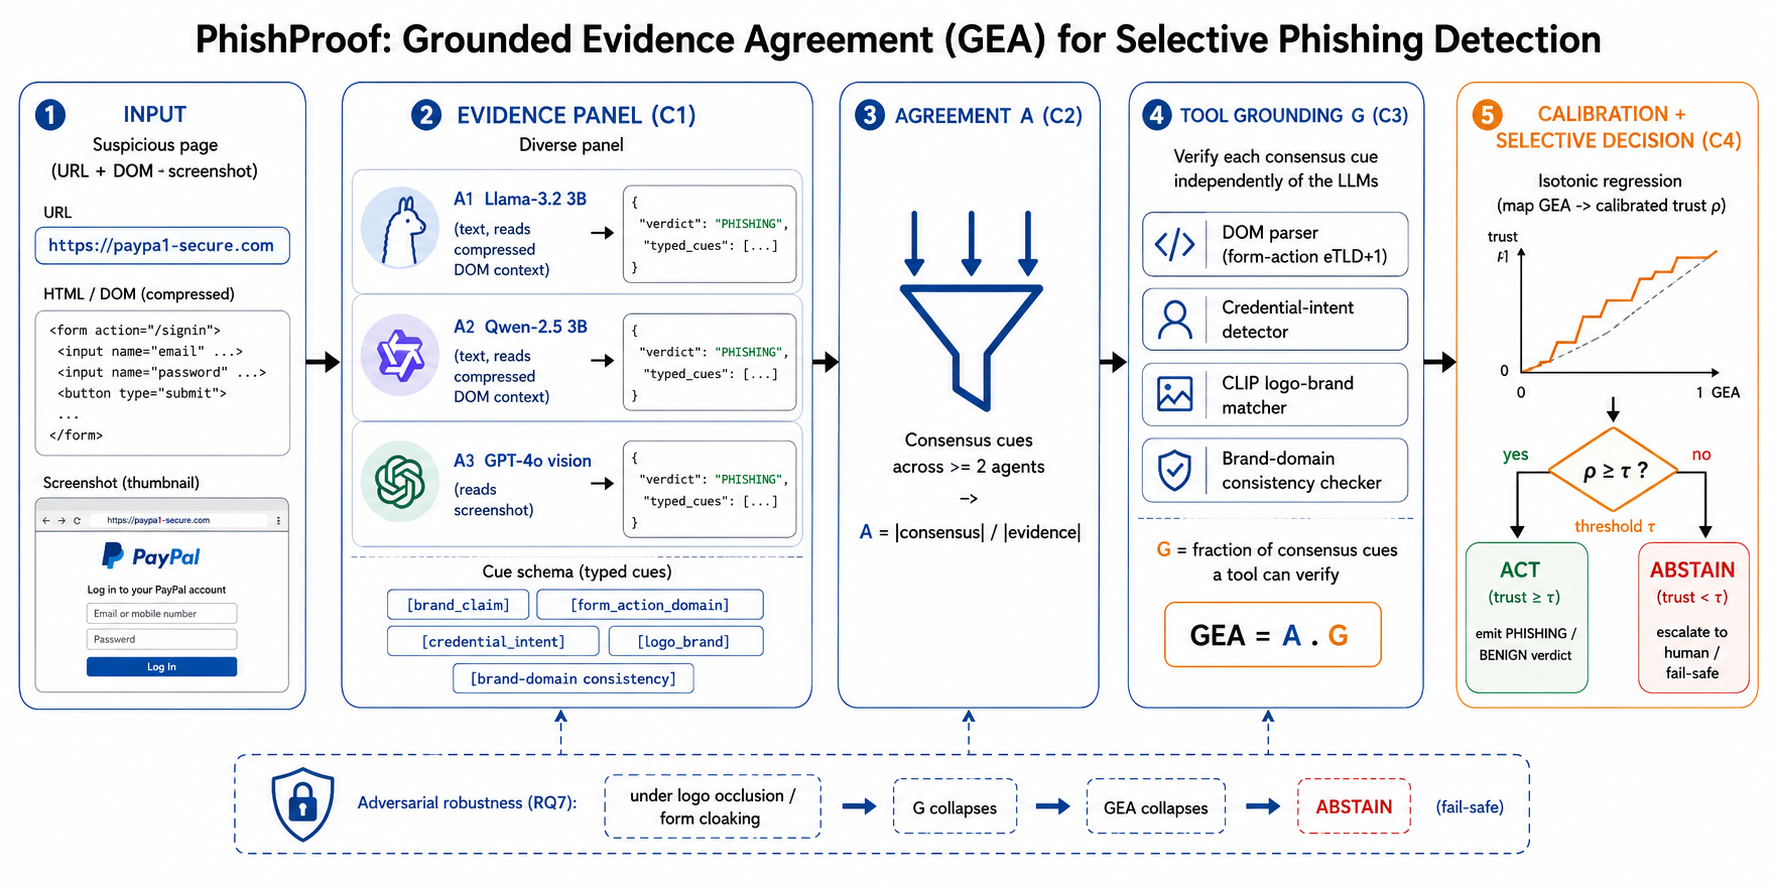
\includegraphics[width=\textwidth]{../figures/fig_overview_visual.png}
\caption{\toolname{} qualitative pipeline. Agents inspect the same page from
complementary views and cite typed evidence cues into a shared set. The system
trusts a verdict only when the agents converge on the same cues and the tool bank
can re-check those cues against the live page. The calibrated selector returns the
label with the verified cues when the evidence is shared and grounded; otherwise it
abstains, including cases where the label vote is plausible but the reasons are thin
or unverified. The threshold and calibrator are set on a held-out labeled split.}
\Description{A four-stage qualitative pipeline. The first panel shows a suspicious
login page and three agents emitting typed evidence cues. The second panel shows a
shared set of typed cues with provenance pins and a highlighted consensus
(agreement A). The third panel shows DOM, brand, consistency, and logo tools re-checking
each consensus cue into a groundedness score G. The final panel forms GEA = A times
G, calibrates it to a probability of correctness on a held-out labeled split, and
acts above a threshold by returning the verified cues or abstains otherwise.}
\label{fig:overview}
\end{figure*}
End-to-end, \toolname{} turns a page into a trusted-and-explained verdict in four
steps, drawn in \autoref{fig:overview} and developed one per subsection in
\autoref{sec:method}; the four components $C_1$--$C_4$ map one-to-one onto these steps.
\textbf{(1)~Investigate.} Each agent plans which signals to examine and calls the
verification tools, emitting its verdict and a set of typed, tool-checkable cues into
the shared cue set ($C_1$ agentic evidence elicitation, \req{1},
\autoref{sec:elicit}).
\textbf{(2)~Aggregate on evidence.} Over the shared set we form the strict-majority
consensus and measure how much of the cited evidence falls within it -- the
evidence-level agreement $\agr$ -- instead of counting how often the verdicts concur
($C_2$, \req{2}, \autoref{sec:agree}).
\textbf{(3)~Verify against the page.} Each consensus cue is re-derived by its tool, and
the groundedness $\grd$ discounts any consensus that the page does not actually bear
out, catching shared hallucinations ($C_3$, \req{3}, \autoref{sec:ground}).
\textbf{(4)~Decide and explain.} The score $\geascore=\agr\cdot\grd$ is calibrated on a
labeled split and thresholded into an act/abstain decision; when it acts it returns the
consensus cues as the explanation, and otherwise escalates the page ($C_4$ calibrated
selection, \autoref{sec:select}). Because the score is a product, a verdict survives to
action only when steps~(2) and~(3) both hold -- precisely guarding against the
right-label/wrong-reason and shared-hallucination failures the label channel misses.

\section{The \texorpdfstring{\toolname}{PhishProof} Detector}
\label{sec:method}

\toolname{} turns the Grounded Evidence-Agreement score of \eqref{eq:gea} into a
calibrated, selective verdict through the four components $C_1$--$C_4$ previewed in
\autoref{sec:form-overview} and drawn in \autoref{fig:overview}. The four subsections
below develop them in the order a page flows through the system -- elicit evidence,
agree on it, ground it, then decide -- after which we give the end-to-end procedure,
its guarantee, and its cost.

\subsection{Evidence agents and the shared cue set}
\label{sec:elicit}
This component produces the per-agent outputs of \eqref{eq:output}. Each member of the
panel is an \emph{evidence agent}: prompted with the page, it \emph{plans} which
signals and modalities to examine, calls the verification tools to obtain them, and
returns a verdict together with the grounded cues it found, drawn from the fixed schema
$\Uschema$ and emitted by constrained decoding as well-typed $(t,v)$ pairs rather than
free text (\req{1}). Constraining the output to the schema is what makes the cue
auditable: it is a typed claim a tool can later re-derive, not prose to be
re-interpreted. The schema is small and auditable -- the brand
claim, the form-action domain, credential intent, the logo brand, a brand--domain
consistency cue derived from the agreed brand and the host, and, where the capture
provides them, the certificate organization and redirect target (both absent in the
corpus of \autoref{sec:experiments}, hence inert there) -- and is shared by every agent, so their cues
are directly comparable. The cues are pooled into the page's \emph{shared cue set},
where each cue is typed, tool-checkable, and tagged with the agent that asserted it, so
the verdict rests on a list of cited, verifiable reasons -- a brand claim paired with
off-brand infrastructure -- rather than an opaque score. Agent \emph{diversity} is a
design choice, not an afterthought: the three agents come from different model families
and at least one is a vision-language model that reads the screenshot, so that
\emph{agreement} on a cue reflects independent corroboration rather than a shared prior
the agents happen to hold (its value is isolated in \autoref{sec:experiments}).

\subsection{Evidence agreement}
\label{sec:agree}
This component scores the shared cue set of \autoref{sec:elicit}. To \emph{aggregate}
and compare cues across agents, two agents must be able to assert the ``same'' cue
despite surface differences, so we first \emph{normalize values}: domains are reduced
to their registrable eTLD+1 and brands to a canonical lexicon entry, so that
``\textsf{paypal-secure.com/login}'' and ``\textsf{paypal-secure.com/signin}'' count as
one form-action cue. On the normalized cues, the consensus set $\cons(\page)$ collects
those a strict majority of the agents assert, and the evidence-level agreement
$\agr(\page)$ of \eqref{eq:agree} is the share of all cues raised that fall in this
consensus (\req{2}). One refinement keeps the rule fair to single-source evidence: a
\emph{perceptual} cue visible to only one modality -- the logo, which only the
vision agent can read -- is admitted to the consensus on its own, since it cannot reach a
majority when a lone agent sees the screenshot; every other type still requires a strict
majority. Agreement is therefore high only when the agents converge on the
\emph{same} evidence, and -- unlike a label-vote concordance -- is unmoved by their
merely concurring on the verdict.

\subsection{Tool-grounding}
\label{sec:ground}
This component verifies the consensus cues from \autoref{sec:agree} against the page.
Agreement alone cannot catch a \emph{shared} hallucination -- a cue the whole panel
asserts but the page does not carry -- so each consensus cue is re-derived from the
page by the tool for its type, $\gver(u,\page)$ (\req{3}). The structural tools verify
deterministically and return $0$ or $1$: the DOM is parsed for the form-action domain,
the certificate for its organization, and the redirect chain for its final target. The
perceptual tool (\textsf{logo-brand}) matches the rendered logo to the claimed brand
and returns a similarity in $[0,1]$. The brand claim is grounded by a check that the page
itself presents the claimed brand; this tool slot can equally be filled by an existing
specialized detector \emph{used as a tool} -- e.g.\ a reference-based visual
matcher~\cite{lin2021phishpedia} or, in principle, an LLM brand-and-domain
checker~\cite{tan2024phishllm}. We verify substitution empirically for the Phishpedia (D1)
matcher: replacing the page-content brand check leaves the selective ranking essentially
unchanged (\autoref{sec:experiments}), so the panel can \emph{subsume} that detector's
signal as a grounding tool rather than re-derive it -- a property we measure for D1 rather
than assume for every specialized detector. The groundedness $\grd(\page)$ of
\eqref{eq:ground} averages these tool outputs over the consensus, and through the
product $\geascore=\agr\cdot\grd$ of \eqref{eq:gea} the score collapses whenever the
agreed evidence does not survive verification. On a clean corpus the agreed cues nearly
always survive that check, so $\grd$ is close to constant and contributes little to the
\emph{ranking} (\autoref{sec:exp_rq3}); its job is to keep the score honest in the
regime the clean corpus lacks, where an attacker corrupts the very cue the panel cites.
There $\grd$ falls, $\geascore$ collapses, and the detector abstains rather than acts on
corrupted evidence -- the fail-safe behaviour we measure directly in
\autoref{sec:exp_adv}.

\subsection{Calibrated selection}
\label{sec:select}
Finally, \toolname{} turns the score $\geascore(\page)$ into an act/abstain decision.
Because phishing labels are available at collection time -- a flagged URL is confirmed
by the public feed it is drawn from~\cite{openphish,phishtank} -- we can set the
operating point on a small held-out labeled split rather than guess it. On that split
we fit a monotonic (isotonic) calibrator $\kappa:\geascore\mapsto\hat\Prob(\hat y = y)$,
which is order-preserving and so leaves the score's ranking -- hence the
risk--coverage curve -- intact while turning it into a probability of correctness, and
we pick the smallest threshold $\thr$ that meets a target selective risk. The detector
then acts with $\hat y(\page)$ when $\geascore(\page)\ge\thr$ and abstains otherwise,
escalating the page to deeper analysis or a human. When it acts, it returns the
consensus cue set $\cons(\page)$ as a verifiable explanation.

\subsection{Procedure, guarantee, and cost}
\label{sec:algo}
\begin{algorithm}[!h]
\caption{\toolname{} inference on a page $\page$}
\label{alg:gea}
\begin{algorithmic}[1]
\State \textbf{for} $m_i\in\panel$: $\ (y_i,\evset_i)\gets m_i(\page)$
       \hfill\Comment{$C_1$ agents call tools, \eqref{eq:output}}
\State $\hat y\gets \mathrm{maj}_i\,y_i$;\ \
       $E\gets\bigcup_i\evset_i$ \hfill\Comment{shared cue set}
\State $\cons\gets\{u: u$ asserted by $>\!M/2$ agents, value-normalized$\}$
\State $\agr\gets \lvert\cons\rvert\,/\,\lvert E\rvert$
       \hfill\Comment{$C_2$, \eqref{eq:agree}}
\State \textbf{for} $u\in\cons$: compute $\gver(u,\page)$;\ \
       $\grd\gets \mathrm{mean}_{u\in\cons}\gver(u,\page)$
       \hfill\Comment{$C_3$, \eqref{eq:ground}}
\State $\geascore\gets \agr\cdot\grd$;\ \ $\hat\rho\gets\kappa(\geascore)$
       \hfill\Comment{\eqref{eq:gea}}
\State \textbf{if} $\geascore\ge\thr$ \textbf{return} $(\hat y,\hat\rho,\cons)$;
       \textbf{else return} $\bot$
\end{algorithmic}
\end{algorithm}

\sstitle{Walk-through}
\autoref{alg:gea} runs the agent panel once, each agent calling its tools to cite its
cues (line~1), takes the majority verdict (line~2), and then does the work that
distinguishes \toolname{} from label-level reliability: it forms the consensus set
(line~3), scores agreement on that evidence rather than on the verdict (line~4),
checks each agreed cue against the page with its tool so a shared hallucination cannot
inflate the score (line~5), and combines the two factors into $\geascore$ (line~6).
Calibration and the selective decision (line~7) then map the score to a trust value and
apply the threshold fitted on the labeled split. The novelty is concentrated in
lines~3--6: the quantity that gates the verdict is grounded agreement on the
\emph{cues}, not concordance of labels, and the returned consensus set is
simultaneously the trust signal and the explanation -- one object serving both
\req{2}--\req{3} and the audit trail of \req{1}.

\sstitle{Guarantee}
Tool-grounding is the component that rules out a shared hallucination inflating the
score, and under one assumption on the tools we can state this precisely.
\begin{assumption}[Tool soundness]\label{ass:sound}
For each cue type, the tool $\gver(u,\page)=1$ if $u$ holds on $\page$ and $0$
otherwise (perceptual types: $\gver(u,\page)$ is the true match score).
\end{assumption}
\begin{proposition}\label{prop:hall}
Under \autoref{ass:sound}, any consensus cue that does not hold on $\page$
contributes $0$ to $\grd(\page)$; hence $\geascore(\page)$ is at most the grounded
fraction of the consensus, and $\geascore(\page)=0$ whenever the entire consensus
is hallucinated.
\end{proposition}
\begin{proof}[Proof sketch]
$\grd$ is the mean of $\gver$ over $\cons$ (\eqref{eq:ground}); by
\autoref{ass:sound} a non-holding cue adds $0$ to that mean, so
$\grd\le\lvert\{u\in\cons: u\text{ holds}\}\rvert/\lvert\cons\rvert$, and
$\geascore=\agr\cdot\grd\le\grd$ inherits the bound. If no consensus cue holds,
$\grd=0$ and thus $\geascore=0$.
\end{proof}
The proposition is modest by design: it bounds, but does not eliminate, gauge error,
since a tool is sound for \emph{what} it checks yet a page can still carry
true-yet-misleading evidence the tool confirms; accordingly we report measured tool
precision and recall against gold in \autoref{sec:experiments} rather than rely on
\autoref{ass:sound} as if it held exactly.

\sstitle{Complexity}
Per page, the cost has two parts: the $M$ agent calls of line~1 -- each a model call
plus the tool calls it issues -- and the verification of the $\lvert\cons\rvert$
consensus cues in line~5. The aggregation steps (lines~2--4,~6) are linear in the
number of cues raised and negligible beside a model call. Each structural tool is an
$\bO(1)$ DOM, certificate, or redirect lookup and the single perceptual check is one
embedding comparison, so verification is $\bO(\lvert\cons\rvert)$ and the per-page cost
is dominated by the $M{=}3$ agent calls; it is independent of the schema size beyond
the cues actually asserted, and there is no training. Relative to the strongest
non-agentic baseline -- a single-model detector -- this is a fixed $M{\times}$ inference
overhead. Selective operation amortizes it: only the abstaining fraction
$1-\phi(\thr)$ is escalated to deeper analysis, so the expected per-page budget is tuned
by the very threshold $\thr$ that sets the risk--coverage operating point
(\autoref{sec:experiments}).

\section{Experiments}
\label{sec:experiments}

We evaluate \toolname{} as a \emph{selective} detector: it may act only on pages
whose evidence is trustworthy enough, and should abstain otherwise. The selective
behavior is the contribution, so the seven questions below probe \emph{when} the
detector should be trusted, how robust that behavior is to its hyperparameters, and
\emph{what} it returns when it acts, rather than raw labelling accuracy:
\begin{compactitem}
\item[(\textbf{RQ1})] Selective detection (\autoref{sec:exp_rq1}): does grounded
evidence-agreement give a better risk--coverage trade-off than label-level
reliability, without sacrificing full-coverage detection accuracy?
\item[(\textbf{RQ2})] Right-label, wrong-reason (\autoref{sec:exp_rq2}): does
\toolname{} flag the pages a panel labels correctly but for the wrong reason --
the pages the reliability baselines act on confidently?
\item[(\textbf{RQ3})] Component attribution (\autoref{sec:exp_rq3}): how much do
evidence-level agreement, groundedness, and panel diversity each contribute?
\item[(\textbf{RQ4})] Calibration (\autoref{sec:exp_rq4}): is the trust score
calibrated, so its reported probability of correctness can be acted on directly?
\item[(\textbf{RQ5})] Sensitivity (\autoref{sec:exp_rq5}): how does the selective
trade-off respond to the two hyperparameters -- panel size and consensus threshold --
and is the default robust?
\item[(\textbf{RQ6})] Explanation (\autoref{sec:exp_rq6}): what does a returned
explanation look like, and does it make the act/abstain decision auditable to an
operator?
\item[(\textbf{RQ7})] Adversarial robustness (\autoref{sec:exp_adv}): when an
attacker corrupts a cited cue -- cloaking the form action or removing the brand logo --
does grounded evidence-agreement \emph{fail safe} (groundedness drops and the detector
abstains) where label-confidence baselines stay overconfident?
\end{compactitem}

\subsection{Setup}
\label{sec:exp_setup}

\sstitle{Benchmark and labels}
We evaluate on \textsc{PhishSel}, a $1{,}330$-page benchmark ($998$ held-out test) built
from the Phishpedia corpus~\cite{lin2021phishpedia}, whose phishing pages were originally
collected from public feeds~\cite{openphish,phishtank}. To make the task
\emph{legitimacy} rather than \emph{page type}, we pair the phishing pages with legitimate
\emph{credential-collection} (login) pages rather than benign homepages -- the latter are
several times larger than the minimal phishing pages and let a model separate the classes
by size alone (see \autoref{sec:limitations}). The phishing half is brand-balanced and
split evenly into easy (unrelated-domain) and hard (brand-in-domain lookalike) pages, the
latter forming the RQ2 subset. Each page carries its URL, DOM, and rendered screenshot;
the corpus does not include TLS certificates or redirect chains, so those two cue types are
inactive and the active schema is \{brand, form-action-domain, credential-intent,
logo-brand\} plus a derived brand--domain consistency check. Labels are available at
collection. We use a class-balanced calibration split ($332$) and a disjoint, balanced test
split ($998$), fit all thresholds and the calibrator on the former, and report every number
on the latter (\autoref{tab:dataset}).
\begin{table}[!h]
\caption{\textsc{PhishSel} composition. Phishing pages are drawn from the Phishpedia
corpus~\cite{lin2021phishpedia} (feeds collected mid-2019--late-2020), brand-balanced and
split evenly into easy (unrelated-domain) and hard (brand-in-domain look-alike) pages
($266$ easy / $233$ hard on the test split); benign pages are credential-collection (login) pages, so
the comparison turns on legitimacy rather than page type. The calibration split fits all
thresholds and the isotonic calibrator; the held-out test split carries every reported
number.}
\label{tab:dataset}
\footnotesize
\setlength{\tabcolsep}{6pt}
\begin{tabular}{lccc}
\toprule
Split & \#pages & \#phishing & \#benign \\
\midrule
Calibration      & \phantom{0,}332 & \phantom{0,}166 & \phantom{0,}166 \\
Test (held-out)  & \phantom{0,}998 & \phantom{0,}499 & \phantom{0,}499 \\
\midrule
Total            & 1{,}330 & \phantom{0,}665 & \phantom{0,}665 \\
\bottomrule
\end{tabular}
\end{table}


\sstitle{Agents, tools, and baselines}
The default panel is $M{=}3$ deliberately diverse \emph{evidence agents}: GPT-4o reading
the screenshot as the vision-language agent, and two different-family text LLMs run
locally -- Llama-3.2-3B (Meta) and Qwen2.5-3B (Alibaba) -- each able to call the
verification tools of \autoref{sec:ground}. The two text agents are deliberately from
different families: RQ3 shows this cross-family diversity, not the agent count, is what
carries the result (\autoref{tab:panel_models} lists the exact models and decoding
settings). All methods receive the same captured page snapshot and no
label at inference time, so any difference reflects how each method scores trust
rather than what information it sees. \toolname{} emits constrained evidence cues
in the schema of \autoref{sec:elicit}, normalizes values as in \autoref{sec:agree},
and verifies only the consensus cues before calibration. We compare against six
reliability baselines, each of which shares this panel or a member of it so that the
comparison isolates \emph{where} agreement is measured:
\begin{compactitem}
\item \emph{(B1) Single-model confidence}~\cite{guo2017calibration}: the strongest
single model with temperature-scaled softmax confidence.
\item \emph{(B2) Verbalized confidence}: the same model asked to state its
confidence.
\item \emph{(B3) Self-consistency}~\cite{wang2023selfconsistency}: the same strongest single
model (GPT-4o), sampled $k{=}5$ times at temperature $0.7$, with the majority-verdict
agreement as the score; run on the full $998$-page test split ($k\times$ API cost).
\item \emph{(B4) Majority vote}~\cite{ensembleornot2024}: panel label agreement.
\item \emph{(B5) Label-agreement}~\cite{dawid1979maximum}: reliability-weighted
label agreement over the panel.
\item \emph{(B6) MultiPhishGuard}~\cite{multiphishguard2025}: a separate GPT-4o
consolidator reads the panel's per-agent verdicts and cited evidence and outputs a
deliberated verdict and confidence, used as the score.
\end{compactitem}
To position \toolname{} against the dedicated phishing literature we also report the
LLM brand-and-domain checker \emph{(D3) PhishLLM}~\cite{tan2024phishllm}, re-run as a
standalone detector on \textsc{PhishSel}. The reference-based matcher \emph{(D1)
Phishpedia}~\cite{lin2021phishpedia} is re-run in a containerized \texttt{detectron2} on the
full test split (\autoref{tab:detect}); \emph{(D2) PhishIntention}~\cite{liu2022phishintention} layers a
heavier credential-page and interaction stage on the same detector core, so we cite its
reported numbers rather than re-running it. In our main runs the brand cue
is grounded by a page-content brand check; we additionally show (\autoref{sec:exp_rq1}) that
a reference detector (D1) can be substituted as this verifier with no loss of ranking, so
the panel \emph{subsumes} its signal directly. Methods that require
\emph{live} counterfactual interaction with the target -- notably DynaPhish's online
reference expansion~\cite{dynaphish2023} -- are out of scope, because that interaction
cannot be replayed on archived snapshots.
\begin{table}[!h]
\caption{The $M{=}3$ evidence-agent panel. The two text agents are deliberately from
different model families and run locally via Ollama on a $16$\,GB laptop (no GPU); the
vision agent is GPT-4o through its API. All agents decode deterministically (temperature
$0$), so the only stochastic choice in the pipeline is the calibration/test partition.}
\label{tab:panel_models}
\footnotesize
\setlength{\tabcolsep}{3.0pt}
\begin{tabular*}{\columnwidth}{@{\extracolsep{\fill}}llllc@{}}
\toprule
Agent & Model & Family & Modality & Host \\
\midrule
$A_1$ & Llama-3.2-3B & Meta    & text   & Ollama (local) \\
$A_2$ & Qwen2.5-3B   & Alibaba & text   & Ollama (local) \\
$A_3$ & GPT-4o       & OpenAI  & vision & API \\
\bottomrule
\end{tabular*}

\footnotesize{Text agents: $8{,}192$-token context, temperature $0$. Vision agent:
\texttt{detail=low}, temperature $0$. The MultiPhishGuard consolidator (B6) and the
verbalized/single-model baselines (B1, B2) reuse GPT-4o.}
\end{table}


\sstitle{Tasks and metrics}
Every method produces a per-page trust score, and we evaluate that score as a
selective detector via \eqref{eq:objective}. The selective metrics are the area
under the risk--coverage curve (\emph{AURC}, selective risk integrated over
coverage); selective accuracy and false-positive rate at $80\%$ coverage
(\emph{SelAcc$_{80}$}, \emph{FPR$_{80}$}); the coverage attainable at $99\%$
selective accuracy (\emph{Cov$_{99}$}), the operating point an operator cares about
most; and the expected calibration error of the trust score (\emph{ECE}). For RQ2 we
add the \emph{flip rate}: the fraction of pages whose panel label changes under a
small evidence-targeted perturbation (a logo morph~\cite{hao2024logomorph} or a
form-action cloak), which measures reason fragility. Because the specialized
detectors carry no abstention mechanism, we also report standard full-coverage
detection quality -- accuracy, precision, recall, and F1 with every page acted on --
so they can be compared at all. We define each abbreviation here and use it
unchanged in every table and figure below.

\sstitle{Protocol}
Operating points are set without touching the test pages: the thresholds for
SelAcc$_{80}$ and Cov$_{99}$ and the isotonic calibrator are all fit on the
calibration split and then applied unchanged to the held-out test split. For RQ2,
each perturbation targets the cited evidence cue while preserving the page's true
label, so a flip measures reason fragility, not a changed ground truth.

\sstitle{Statistical reporting}
Numeric cells report mean$_{\pm\text{95\% CI}}$ from a paired bootstrap over pages
(all methods share the same page draws). At $998$ test pages the intervals are wide, so
we describe a difference as significant only when the intervals do not overlap and as
suggestive otherwise; we are explicit about which is which in the text. The proposed
method is \textbf{bold} and the best baseline is \underline{underlined} in every table.
As the panel runs at temperature $0$ (deterministic given a page), the only stochastic
choice is the calibration/test partition; to confirm the headline is not an artifact of one
draw, we re-partition the $1{,}330$ pages five ways (stratified $75/25$) and refit the
calibrator each time. The metrics are stable across splits -- AURC $1.8\pm0.2$,
SelAcc$_{80}$ $97.5\pm0.3$, ECE $0.018\pm0.006$, Cov$_{99}$ $0.29\pm0.04$ -- and on AURC,
selective accuracy, and coverage the split reported in \autoref{tab:main} sits among the more
conservative draws (its ECE, $0.015$, is marginally better than the cross-split mean).

\sstitle{Run environment and cost}
The two text agents run locally on a 16\,GB commodity laptop via Ollama (no GPU) at
temperature $0$; the vision agent and the consolidator are GPT-4o through its API; the
DOM, redirect, logo (CLIP), and calibration code are CPU-only. Every model call is cached,
so the comparison is reproducible and re-scoring variants (the ablations) needs no
re-running. We log prompts, raw agent outputs, value-normalized cues, tool results,
thresholds, and per-page trust scores, and release the schemas, prompts, tool wrappers,
calibration code, and figure-generation scripts. \toolname{} has no training phase: per
page it runs the $M{=}3$ agents plus the cheap tool checks. \autoref{tab:cost} gives the
per-page budget: the panel's API cost is dominated by a single GPT-4o vision call
($\approx\$8$ per $1{,}000$ pages), since the two text agents run locally for free, so
\toolname{} fits a commodity $16$\,GB laptop with no GPU. The $M{=}3$ panel is a fixed
$3\times$ model-call overhead over a single-model detector (\autoref{fig:pareto}), amortized
because only the abstaining fraction $1-\phi(\thr)$ is escalated. At that budget \toolname{} stays
level with the panel baselines while reaching markedly higher deployable coverage,
and it dominates the five-sample self-consistency baseline (B3, \autoref{tab:main}: AURC
$5.1$ vs.\ $2.3$, and Cov$_{99}{=}0$ -- it never reaches the $99\%$-accuracy operating point)
at one-fifth its API cost, since B3 issues five GPT-4o vision calls per page where \toolname{}
issues one. Resampling one strong model improves selective accuracy over single-call B1/B2 but
does not cure its overconfidence: on the visually convincing brand replicas that dominate the
corpus, the model is confidently wrong and the five samples agree on the wrong \textsf{benign}
verdict, which is precisely the label-level trust that grounded agreement is designed to
replace.
\begin{table}[!h]
\caption{Per-page compute budget. The panel uses two local 3B text agents (free, on the
$16$\,GB laptop) and one GPT-4o vision call, so API cost is dominated by that single call;
the two text agents add no API cost. Dollar cost is at GPT-4o list price with detail-low
images; latency is indicative wall-clock on the CPU-only laptop (providers' API latency is
not controlled by us). The $M{=}3$ panel is a fixed $3\times$ model-call overhead over a
single-model detector, amortized by abstaining on the $1-\phi(\thr)$ fraction.}
\label{tab:cost}
\footnotesize
\setlength{\tabcolsep}{5pt}
\begin{tabular}{lccc}
\toprule
Method & Calls/page & API \$/1k & Latency/page \\
\midrule
\textbf{\toolname{}} (panel)    & 3 (2 local\,+\,1 API) & $\approx$8 & $\approx$20\,s \\
\;\,+\,B6 consolidator          & +1 API                & +$\approx$3 & +$\approx$3\,s \\
D3 PhishLLM                     & 1 API                 & $\approx$5 & $\approx$4\,s \\
D1 Phishpedia                   & 0 (local CPU)         & 0          & $\approx$15\,s \\
B1/B2 single-model              & 1                     & $\approx$2 & $\approx$3\,s \\
B3 Self-consistency ($k{=}5$)   & 5 API (same model)    & $\approx$40 & $\approx$15\,s \\
\bottomrule
\end{tabular}
\end{table}

% Generated PNG. Source: figures/gen_experiment_figs.py
% Regenerate: uv run --with matplotlib --with numpy python figures/gen_experiment_figs.py
\begin{figure}[!h]
\centering
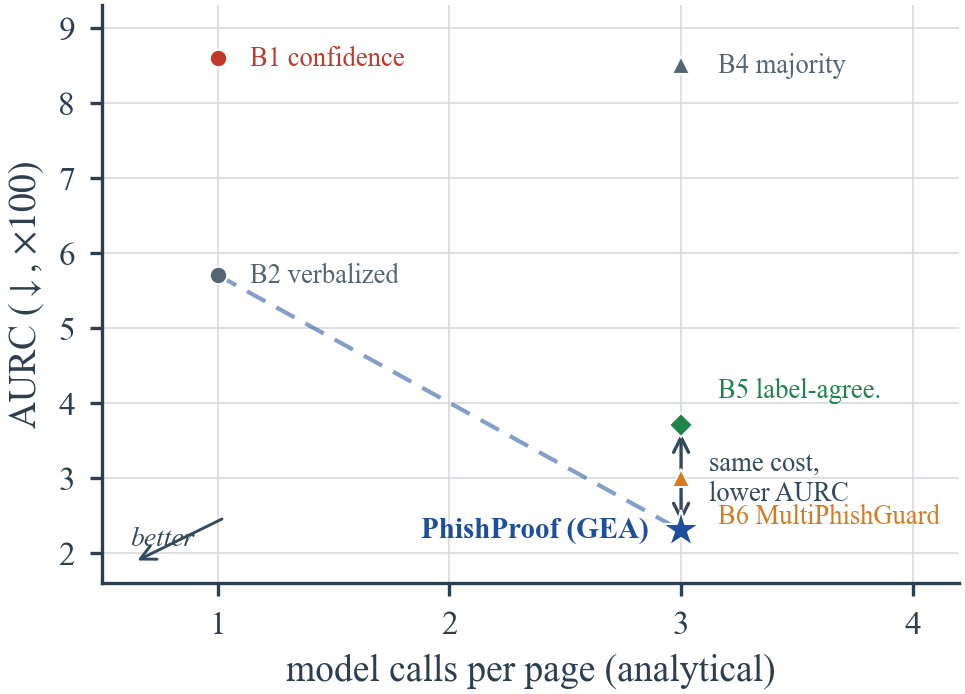
\includegraphics[width=\linewidth]{fig_pareto}
\caption{Cost--quality trade-off: per-page model calls (analytical) versus AURC
($\downarrow$). At the $M{=}3$ panel's call budget \toolname{} has the lowest AURC in point
estimate (on par with B6 within CI),
below the other three-call panel methods (B4/B5/B6) and far below the single-call
confidence read-outs.}
\Description{A scatter plot of AURC against per-page model calls. PhishProof sits at
the bottom of the cost-quality frontier: at three model calls it has lower AURC than
the label-agreement, majority-vote, and MultiPhishGuard baselines at the same cost,
and far lower than the single-call confidence baselines.}
\label{fig:pareto}
\end{figure}


\sstitle{Reproducibility}
The pipeline is deterministic given the page snapshots and the dataset partition. We pin the
exact artifacts so the headline numbers can be regenerated: the panel is
\autoref{tab:panel_models} (Llama-3.2-3B and Qwen2.5-3B via Ollama, GPT-4o via API, all at
temperature $0$); the calibration and test splits are released with SHA-256 checksums
(\texttt{calibration.jsonl} \texttt{9f2c9bb8\dots}, \texttt{test.jsonl} \texttt{391fc594\dots});
the code runs on CPython $3.14$ with CPU-only DOM, CLIP, and calibration code. Every model
call is content-hash cached, so all ablations and the design-justification probes
(\autoref{sec:exp_negatives}) re-score from cache without re-running any agent. We release
the cue schema and prompts, the tool wrappers, the calibrator and threshold-fitting code,
and the figure- and table-generation scripts. Code, manifests, and headline result files are
available at \url{https://github.com/phamhyta/phishproof}; page snapshots and the full agent
cache are archived separately (Zenodo DOI upon acceptance).

\sstitle{Tool soundness}
\autoref{prop:hall} assumes the tools are sound (\autoref{ass:sound}); we check this for
\emph{every} active verifier, not only the brand check, by scoring each tool as a detector of
an independently-derivable target property (\autoref{tab:verifier_soundness}). The two
deterministic structural verifiers are reliable: the form-action verifier reproduces the
DOM-parsed action domains exactly (recall and specificity $1.00$), and the credential
verifier never misses a real password field (recall $1.00$). The two reference/perceptual
verifiers are accurate but soft: the brand-grounding tool recovers the impersonated gold
brand on $87.6\%$ of pages and spuriously grounds an absent brand on only $5\%$ ($95\%$
specificity), while the CLIP logo tool matches the gold brand at $89.0\%$ but grounds a
\emph{wrong} brand $34\%$ of the time (specificity $0.66$). Two soundness gaps are thus
explicit: the credential verifier over-fires on hint-only fields (precision $0.62$), and the
CLIP logo verifier is a soft matcher. Both are consistent with \autoref{prop:hall}
\emph{bounding} rather than eliminating gauge error, and the residual recall/precision gaps
are one reason groundedness is conservative on this corpus.
\begin{table}[!h]
\caption{Per-cue-type verifier soundness. Each grounding tool is scored as a detector of an
independently-derivable target property on the 998-page test split: the brand and logo
verifiers against the dataset brand annotation (specificity uses a random wrong brand), the
form-action verifier against the DOM-parsed action domains, and the credential verifier
against the strict presence of an \texttt{<input type=password>} field. The deterministic
structural verifiers are exact (form-action) or high-recall (credential), while the
perceptual CLIP logo verifier is a \emph{soft} matcher (specificity $0.66$). The
credential verifier never misses (recall $1.0$) but over-fires on hint-only fields
(precision $0.62$).}
\label{tab:verifier_soundness}
\footnotesize
\setlength{\tabcolsep}{3.0pt}
\begin{tabular*}{\columnwidth}{@{\extracolsep{\fill}}llcccc@{}}
\toprule
Cue type & Verifier & Prec. & Recall & Spec. & $n$ \\
\midrule
\texttt{brand\_claim}        & HTML-brand   & ---   & 0.876 & 0.950 & 499 \\
\texttt{form\_action\_domain} & DOM form     & ---   & 1.000 & 1.000 & 1067 \\
\texttt{credential\_intent}   & DOM cred.    & 0.624 & 1.000 & ---   & 998 \\
\texttt{logo\_brand}          & CLIP ViT-B/32 & ---  & 0.890 & 0.660 & 200 \\
\bottomrule
\end{tabular*}

\footnotesize{Specificity $=1-$ false-grounding rate against a random wrong value. The
logo verifier is subsampled to 200 pages with a detected logo box; others use the full
applicable split.}
\end{table}


\subsection{Selective Detection}
\label{sec:exp_rq1}

\sstitle{Full-coverage detection accuracy}
To answer \textbf{RQ1} we first establish the floor: at full coverage \toolname{} is a
solid detector, so its trust layer sits on top of -- not in place of -- accurate
labelling. \autoref{tab:detect} reports full-coverage quality with every page acted on.
\toolname{} reaches $91.9\%$ accuracy and $91.3$ F1 at very high precision ($98.8\%$),
ahead of the re-run LLM checker D3 ($83.7\%$ / $81.6$); but \toolname{} is an $M{=}3$
panel under a majority vote while D3 is a single model, so this margin reflects
ensembling as much as the trust layer, and we make no detector-leaderboard claim. The
re-run reference matcher D1 (Phishpedia, $n{=}998$) trails on F1 ($76.6$)
at high precision ($94.2$): it fires only on confident logo matches against its
reference list and abstains on the rest, so its recall ($64.5$) is bounded by brand
coverage; D2 adds a heavier stage on the same core and is cited. Beyond a competitor, D1
also serves as a \emph{grounding tool}: substituting it for the page-content brand check
leaves the selective ranking essentially unchanged (AURC $2.33$ vs.\ $2.29$ on the full
$998$ pages), so the panel can invoke a specialized detector to ground its brand cue
rather than re-derive it -- the ``subsumes the detector'' property of \autoref{sec:method},
measured here for D1 only (D3 substitution as a grounding tool is left to future work).
The intended reading is
only that detection is not sacrificed for the abstention and explanation the rest of the
section measures.
\begin{table}[!h]
\caption{Full-coverage detection quality on \textsc{PhishSel} (no abstention).
\toolname{} (the $M{=}3$ panel under a majority vote) and D1--D3 are re-run on the
full $998$-page test split (mean$_{\pm\text{95\% CI}}$, paired bootstrap).
D1 Phishpedia uses a containerized \texttt{detectron2} reference matcher ($\sim$15\,s/page on CPU).
D2 PhishIntention adds a heavier credential-page and interaction stage on the same detector
core, so we cite its reported results. \toolname{} leads the re-run reference detector D1
and the LLM checker D3 on accuracy and F1, but it is a three-model panel against a single
LLM checker, so the margin reflects ensembling as much as the trust layer; the point is that
detection is not sacrificed for the abstention and explanation the rest of the section
measures.}
\label{tab:detect}
\footnotesize
\setlength{\tabcolsep}{4.0pt}
\begin{tabular}{lcccc}
\toprule
Detector & Acc$\uparrow$ & Prec.$\uparrow$ & Rec.$\uparrow$ & F1$\uparrow$ \\
\midrule
D1 Phishpedia~\cite{lin2021phishpedia}        & 80.3$_{\pm2.6}$ & 94.2$_{\pm2.4}$ & 64.5$_{\pm4.3}$ & 76.6$_{\pm3.3}$ \\
D2 PhishIntention~\cite{liu2022phishintention} & \multicolumn{4}{c}{cited (heavier CRP/interaction stage); see \cite{liu2022phishintention}} \\
D3 PhishLLM~\cite{tan2024phishllm}             & 83.7$_{\pm2.4}$ & 93.3$_{\pm2.6}$ & 72.5$_{\pm4.1}$ & 81.6$_{\pm2.8}$ \\
\midrule
\textbf{\toolname{}} (full cov., $n{=}998$)   & \textbf{91.9}$_{\pm1.7}$ & \textbf{98.8}$_{\pm1.0}$ & 84.8$_{\pm2.5}$ & \textbf{91.3}$_{\pm1.7}$ \\
\bottomrule
\end{tabular}
\end{table}


\sstitle{Risk--coverage and deployment coverage}
Scoring agreement on grounded evidence, rather than on labels, gives the best selective
trade-off on the headline metrics. \autoref{tab:main} reports the comparison and
\autoref{fig:riskcoverage} the curves: \toolname{} has the lowest AURC ($2.3$, a
$38\%$ reduction over the label-agreement baseline B5), the highest selective accuracy
at $80\%$ coverage ($97.0\%$), and by a clear margin the best-calibrated trust score
(ECE $0.015$ versus $\ge0.026$ for every baseline). With $998$ test pages the bootstrap
intervals are wide, so the AURC lead over the strongest baseline (B6 MultiPhishGuard,
$3.0$) is suggestive rather than statistically separated (paired $\Delta$AURC $-0.4$, $95\%$
CI $[-1.5,+0.8]$, $p=0.44$). The direction, however, is robust to how the test set is
partitioned: \toolname's AURC is the lower of the two on $21/21$ $70\%$ subsamples and on
$4/5$ stratified folds, so the lead is consistent in sign even where it is underpowered to
separate. The calibration and selective-accuracy gaps are
unambiguous (paired $\Delta$ECE $-0.066$, CI $[-0.088,-0.043]$; $\Delta$SelAcc$_{80}$
$+2.4$, CI $[+1.0,+3.9]$). The deployment number Cov$_{99}$ is the one metric a baseline wins:
B6 reaches $0.36$ against \toolname's $0.25$, because grounded evidence is sparse on the
many correctly-labelled-but-weakly-grounded benign pages, which \toolname{} ranks low
and therefore abstains on. All panel-based methods meet at the shared full-coverage
panel error -- \toolname{} does not change the majority label, only the order in which
pages are trusted. The decisive comparison is against the label-aggregation baselines
(B4, B5): they carry a high ECE ($0.25$) because a label-vote share is not a calibrated
trust signal, whereas \toolname{} reads agreement on \emph{grounded evidence}, which is
where the calibration and AURC gains come from -- not merely from polling several models.
\begin{table}[!h]
\caption{RQ1. Selective detection on \textsc{PhishSel} (998 test pages). Lower
AURC/FPR/ECE and higher SelAcc/Cov are better. Cells are mean$_{\pm\text{95\% CI}}$
from a paired bootstrap over pages; \textbf{best}, \underline{best baseline}. The
$\Delta$ row is relative to B5. \toolname's gains in ECE and SelAcc$_{80}$ over the best
baseline are statistically significant (paired bootstrap CI excludes zero, marked
$\ast$); its AURC lead over B6 is the best point estimate but not statistically separated.
Self-consistency (B3) is the same strongest single model (GPT-4o) resampled $k{=}5$ times at
temperature $0.7$; its row is a point estimate ($k\times$ cost, no bootstrap CI).}
\label{tab:main}
\footnotesize
\setlength{\tabcolsep}{2.6pt}
\resizebox{\columnwidth}{!}{%
\begin{tabular}{lccccc}
\toprule
Method & AURC$\downarrow$ & SelAcc$_{80}\uparrow$ & FPR$_{80}\downarrow$ & Cov$_{99}\uparrow$ & ECE$\downarrow$ \\
\midrule
B1 Single-model conf.\         & 8.6$_{\pm2.4}$ & 92.4$_{\pm1.9}$ & 1.0$_{\pm0.9}$ & 0.00$_{\pm0.02}$ & 0.081$_{\pm0.017}$ \\
B2 Verbalized conf.\           & 5.7$_{\pm1.5}$ & 92.4$_{\pm1.8}$ & 0.9$_{\pm1.1}$ & 0.26$_{\pm0.03}$ & 0.026$_{\pm0.016}$ \\
B3 Self-consistency           & 5.1 & 96.0 & 0.4 & 0.00 & 0.041 \\
B4 Majority vote               & 8.5$_{\pm2.4}$ & 92.4$_{\pm1.9}$ & 1.0$_{\pm0.9}$ & 0.00$_{\pm0.02}$ & 0.252$_{\pm0.017}$ \\
B5 Label-agreement             & 3.7$_{\pm1.2}$ & 93.6$_{\pm1.8}$ & 1.5$_{\pm1.3}$ & 0.10$_{\pm0.23}$ & 0.238$_{\pm0.017}$ \\
B6 MultiPhishGuard             & \underline{3.0}$_{\pm1.1}$ & \underline{94.6}$_{\pm1.6}$ & 1.5$_{\pm1.3}$ & \underline{0.36}$_{\pm0.24}$ & \underline{0.083}$_{\pm0.016}$ \\
\textbf{\toolname{} (GEA)}     & \textbf{2.3}$_{\pm0.9}$ & \textbf{97.0}$^{\ast}_{\pm1.2}$ & \textbf{1.3}$_{\pm1.1}$ & \textbf{0.25}$_{\pm0.15}$ & \textbf{0.015}$^{\ast}_{\pm0.013}$ \\
\midrule
$\Delta$ vs B5                 & $-38\%$ & $+3.4$ & $-0.2$ & $+0.15$ & $-0.22$ \\
\bottomrule
\end{tabular}%
}
\end{table}

% Generated PNG. Source: figures/gen_experiment_figs.py
% Regenerate: uv run --with matplotlib --with numpy python figures/gen_experiment_figs.py
\begin{figure}[!h]
\centering
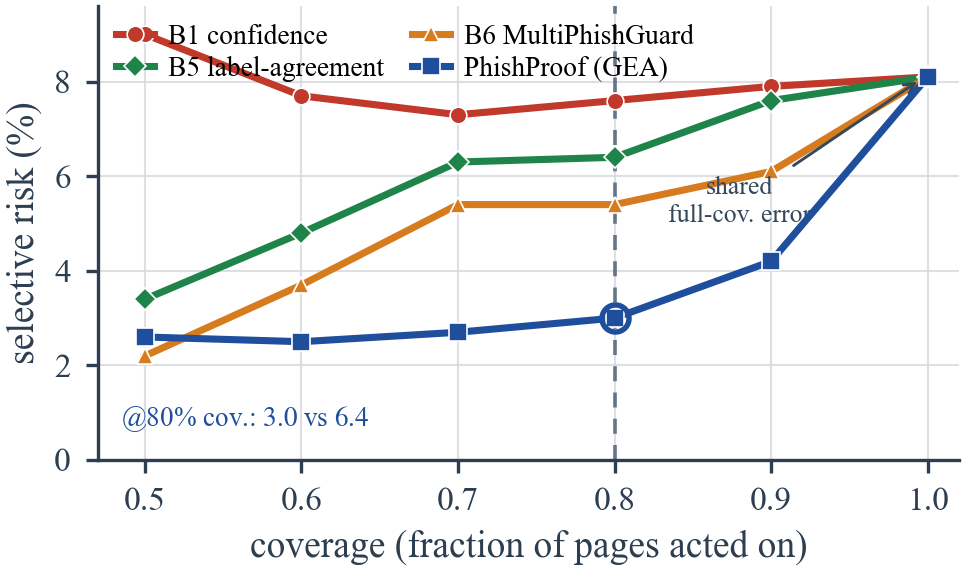
\includegraphics[width=\linewidth]{fig_riskcoverage}
\caption{Risk--coverage on \textsc{PhishSel} (RQ1, 998 pages). Lower selective risk is
better; the ring marks $80\%$ coverage. All panel methods meet at the shared
full-coverage error ($8.1\%$); \toolname{} changes only the abstention order and has
low risk as coverage tightens (best point-estimate AURC, on par with B6 within CI;
decisively the best calibration and selective accuracy).}
\Description{A line chart of selective risk versus coverage. PhishProof has the lowest
risk curve as coverage tightens and among the lowest area under the curve among the plotted
methods, which all meet at the shared full-coverage error.}
\label{fig:riskcoverage}
\end{figure}


\sstitle{Failure modes}
At full coverage \toolname{} errs on $81$ of $998$ pages, almost all in one direction:
$76$ are missed phishing pages and only $5$ are false alarms, matching the high-precision,
lower-recall profile of \autoref{tab:detect}. The misses are evidence-poor by construction:
$96\%$ carry no agreed brand cue and $66\%$ reach no consensus at all -- minimal or
hard-to-read pages on which the panel never converges. Crucially, the trust score
\emph{knows} this: errors carry a mean $\geascore$ of $0.20$ against $0.62$ on correct pages,
so the selective layer abstains on most of them and only $15$ of the $81$ errors are
\emph{confident} ($\geascore>0.5$). The dominant failure is thus a safe one -- abstention on
a page whose evidence does not cohere -- rather than a confident wrong verdict, which is the
behaviour the selective design is meant to produce. \autoref{tab:failure_modes} breaks the
errors down: the only genuinely dangerous mode -- a confident missed-phish that carries an
agreed brand cue -- accounts for just $3$ of $998$ pages.
\begin{table}[!h]
\caption{Failure-mode taxonomy of the $81$ full-coverage errors on the $998$-page test
split. Almost all errors are evidence-poor missed phishing pages on which the panel never
converges, and they carry a low mean $\geascore$ -- so the selective layer abstains on them.
Only $15$ of the $81$ errors are \emph{confident} ($\geascore{>}0.5$), and just $3$ are
confident missed-phish with an agreed brand cue (the only truly dangerous mode). Correct
pages average $\geascore{=}0.62$ for comparison.}
\label{tab:failure_modes}
\footnotesize
\setlength{\tabcolsep}{3.0pt}
\begin{tabular*}{\columnwidth}{@{\extracolsep{\fill}}lccc@{}}
\toprule
Failure mode & $n$ & mean $\geascore$ & confident ($>0.5$) \\
\midrule
FN: no consensus cue        & 50 & 0.00 & 0 \\
FN: cues but no brand       & 23 & 0.46 & 8 \\
FN: brand in consensus      & 3  & 0.81 & 3 \\
FP: false alarm             & 5  & 0.67 & 4 \\
\midrule
All errors                  & 81 & ---  & 15 \\
\bottomrule
\end{tabular*}
\end{table}


\subsection{Right-Label, Wrong-Reason Pages}
\label{sec:exp_rq2}
\textbf{RQ2} asks whether low GEA flags pages the panel labels correctly but for a
fragile reason -- the right-label, wrong-reason (RLWR) case. We test this with a small
evidence-targeted perturbation (a form-action cloak that rewrites the cited form to an
on-brand domain) that preserves the page's true label, and measure how often the panel
verdict flips. The effect is present but \emph{modest and benchmark-dependent}, and we
report it as such. On the unrestricted test split, where every phishing page sits on an
obviously off-brand host, verdicts are stable regardless of GEA and the gradient is
essentially flat. The RLWR effect only appears on the harder \emph{lookalike} subset
(brand-in-domain hosts such as \textsf{steamcoommuniity.com}; $233$ hard pages in test,
$n{=}200$ correctly labelled by the panel), and even there it is small:
\autoref{tab:rlwr} bins these correctly-labelled pages into GEA quintiles, and
fragility concentrates in the lowest quintile ($12\%$ flip) against $\le5\%$ above it.
Split coarsely by GEA level instead, the low-GEA group ($\geascore{<}0.5$, $n{=}98$) flips
$7.1\%$ against $6.0\%$ for the high-GEA group ($\geascore{>}0.72$, $n{=}67$) -- an overall
gap of only $1.2\times$, modest precisely because the effect is concentrated in the lowest
bin rather than spread across the range. So GEA
does rank the most fragile lookalike verdicts lowest -- which is the direction RQ2
predicts and the behaviour an operator wants from the abstention -- but the sharp
partition the illustrative design assumed does not materialise on this benchmark, whose
phishing pages carry few shared hallucinations for grounding to catch. We treat this as
a limitation of the benchmark rather than evidence against the mechanism
(\autoref{sec:limitations}). A natural \emph{evasive} subset isolates the effect more
clearly: filtering the $423$ correctly-labelled phish for pages with a minimal DOM
($<\!5$\,KB) or no detectable logo region yields $72$ pages, the closest the corpus
comes to logo-free/minimal-cue phishing. On this evasive subset the form-action cloak
flips $12.5\%$ of verdicts against $5.4\%$ on the rest ($2.3\times$), logo occlusion
$15.9\%$ vs.\ $8.3\%$ ($1.9\times$), and the white-box all-cue attack $19.4\%$ vs.\
$7.7\%$ ($2.5\times$) -- in every case the GEA-fragile pages are the ones a small
evidence-corruption flips. The mechanism is real; on a corpus richer in such pages the
flat-on-clean gradient would resolve into the sharp partition the design predicts.
\begin{table}[!h]
\caption{RQ2. Correctly labeled \emph{lookalike} phishing pages (brand-in-domain hard
subset: $n{=}200$ correctly labeled pages of $233$ hard pages in the test split) binned into
GEA quintiles. ``Flip'' is the label-flip rate under a
small evidence-targeted perturbation (form-action cloak) that preserves the true label.
Fragility is concentrated in the lowest-GEA bin ($12\%$ vs $\le5\%$ above it); a coarser
split by GEA \emph{level} -- the low group ($\geascore{<}0.5$, $n{=}98$) vs the high group
($\geascore{>}0.72$, $n{=}67$) -- gives a modest $7.1\%$ vs $6.0\%$ ($1.2\times$), small
because the effect is concentrated in the lowest bin rather than spread. On the
unrestricted test split, where the off-brand signal is unambiguous, the gradient is
flat. The strong right-label-wrong-reason effect is thus benchmark-dependent (see
Limitations), not the dramatic split the illustrative design assumed.}
\label{tab:rlwr}
\footnotesize
\setlength{\tabcolsep}{4.0pt}
\begin{tabular*}{\columnwidth}{@{\extracolsep{\fill}}lcc@{}}
\toprule
GEA quintile (low $\to$ high) & mean GEA & Flip$\downarrow$ \\
\midrule
Q1 (lowest)  & 0.29 & 12\% \\
Q2           & 0.50 & 2.5\% \\
Q3           & 0.55 & \phantom{0}5\% \\
Q4           & 0.72 & \phantom{0}5\% \\
Q5 (highest) & 0.92 & \phantom{0}5\% \\
\bottomrule
\end{tabular*}
\end{table}


\subsection{Component Ablation}
\label{sec:exp_rq3}
\emph{Panel diversity} is the load-bearing component: \autoref{tab:ablation} removes one
piece at a time. By far the largest effect is removing cross-family diversity -- swapping
the two distinct-family text agents for two same-family ones while holding the count at
$M{=}3$: on the matched subset this raises AURC from $1.3$ to $27.5$ and drops even
full-coverage accuracy from $0.90$ to $0.68$, because two same-family agents make
correlated errors that outvote the lone vision agent. This is why \emph{diversity}, not
panel size, is the design variable. Replacing evidence-level agreement with the label-vote
share costs the next most ($2.3\to3.5$ AURC, approaching the label-agreement baseline B5
($3.7$) of \autoref{tab:main}), confirming that the selective gain comes from scoring agreement on
evidence rather than on labels. Removing the calibrator leaves the \emph{ranking} intact
(AURC unchanged) but inflates the trust score's ECE from $0.015$ to $0.331$: calibration
governs the reported probability, not the order -- exactly the split of duties RQ4
examines. Dropping groundedness, by contrast, barely moves AURC ($2.3\to2.1$): on this
benchmark the agreed cues almost always survive their tool check, so there are few shared
hallucinations for $\grd$ to discard and grounding contributes little to the
\emph{ranking}. Its role is the guarantee of \autoref{prop:hall} and the verifiability of
the returned explanation rather than a measurable AURC gain here -- a point we return to
in \autoref{sec:limitations} and demonstrate directly under adversarial cue corruption in
\autoref{sec:exp_adv}, where groundedness is what drives the detector to abstain.
\begin{table}[!h]
\caption{RQ3. Component ablation. AURC/FPR$_{80}$ ($\times100$) and ECE; lower is
better. The first four rows are on the full 998-page test split; the calibrated ECE
of each row is reported (the $-$calibration row uses the raw, un-calibrated score).
The $-$diversity row is on a 100-page subset on which the full diverse panel scores
AURC $1.3$, so swapping the cross-family text agents for two same-family ones raises
AURC to $27.5$ and full-coverage accuracy falls $0.90\!\to\!0.68$ -- by far the
largest effect, which is why \emph{diversity}, not panel size, is the design variable.
The GPT-4o vision agent is held fixed in both arms, so the row isolates the effect of
cross-family \emph{text} diversity rather than confounding it with a change of vision model.}
\label{tab:ablation}
\footnotesize
\setlength{\tabcolsep}{3.0pt}
\begin{tabular*}{\columnwidth}{@{\extracolsep{\fill}}lccc@{}}
\toprule
Variant & AURC$\downarrow$ & FPR$_{80}\downarrow$ & ECE$\downarrow$ \\
\midrule
\textbf{\toolname{} (full)}                       & \textbf{2.3} & \textbf{1.3} & \textbf{0.015} \\
\;$-$ calibration                                  & 2.3 & 1.3 & \underline{0.331} \\
\;$-$ groundedness $\grd$ (\req{3})                & 2.1 & 1.2 & 0.014 \\
\;$-$ evidence-level $\agr$ (\req{2})              & \underline{3.5} & 1.3 & 0.015 \\
\;$-$ diversity (same-family)\textsuperscript{$\dagger$} & \underline{27.5} & \underline{48.6} & --- \\
\bottomrule
\end{tabular*}

\footnotesize{\textsuperscript{$\dagger$}100-page subset; the diverse panel scores
AURC $1.3$ on the same pages.}
\end{table}


\subsection{Why a Parameter-Free, Small-Model Design? Negative Results for Plausible Extensions}
\label{sec:exp_negatives}
The ablation shows which components are load-bearing; a natural follow-up is whether several
``obvious'' extensions improve on the deliberately simple design. We probe each -- four by
re-scoring the cached agent outputs at no extra cost, and one by re-running the panel with
larger models -- and find that the parameter-free product $\agr\!\cdot\!\grd$ over a fixed,
diverse, small-model panel is hard to beat.

\sstitle{A learned aggregator does not beat the crisp product}
The fusion $\geascore{=}\agr\!\cdot\!\grd$ has no learned parameters. We ask whether learning
a combiner over the per-cue-type signals $(a_t,g_t)$ -- which expose more structure than the
two scalars $\agr,\grd$ -- lowers AURC. \autoref{tab:hfgea} fits four combiners of increasing
capacity on the same $332$-page calibration split: a weighted geometric mean, a $2$-additive
Choquet integral, a per-type logistic model, and a Takagi--Sugeno--Kang fuzzy system. None
improves the headline ranking metric. The high-capacity fuzzy and Choquet models
\emph{overfit} the small calibration split (AURC $3.9$--$4.4$, Cov$_{99}$ collapsing to
$0.01$); the only competitive learned model, logistic regression, merely trades a small
AURC loss ($2.5\to2.9$) for a marginal Cov$_{99}$/FPR$_{80}$ gain. The crisp product remains
best on AURC ($2.5$) and ECE ($0.015$), so we keep it and read this as evidence that the
calibration-scale data does not support a learned fusion.
\begin{table}[!h]
\caption{Does a \emph{learned} aggregator beat the parameter-free $\agr\!\cdot\!\grd$?
Each combiner is fit on the 332-page calibration split over the same per-cue-type
$(a_t,g_t)$ signals (four active types) and evaluated on the 998-page test split.
AURC/SelAcc$_{80}$/FPR$_{80}$ are $\times100$. No learned combiner improves the headline
ranking metric (AURC): the high-capacity fuzzy/Choquet models overfit the small
calibration split (AURC $3.9$--$4.4$, Cov$_{99}$ collapses), and the only competitive
learned model (logistic) merely trades AURC for a small Cov$_{99}$/FPR gain. The crisp
product remains best on AURC and ECE, justifying the parameter-free design.}
\label{tab:hfgea}
\footnotesize
\setlength{\tabcolsep}{3.0pt}
\begin{tabular*}{\columnwidth}{@{\extracolsep{\fill}}lccccc@{}}
\toprule
Aggregator & AURC$\downarrow$ & SelAcc$_{80}\uparrow$ & FPR$_{80}\downarrow$ & Cov$_{99}\uparrow$ & ECE$\downarrow$ \\
\midrule
\textbf{crisp $\agr\!\cdot\!\grd$ + iso} & \textbf{2.47} & 96.87 & 1.27 & 0.210 & \textbf{0.015} \\
weighted geom. $\agr^a\grd^b$            & 2.56 & 97.12 & 1.20 & 0.210 & --- \\
Choquet 2-additive                       & 4.44 & 94.49 & 1.34 & 0.012 & 0.249 \\
logistic (per-type)                      & 2.85 & 97.12 & \textbf{0.97} & \textbf{0.228} & 0.020 \\
TSK fuzzy (heavy $L_2$)                  & 3.89 & 96.24 & 1.30 & 0.012 & 0.115 \\
\bottomrule
\end{tabular*}

\footnotesize{All aggregators are compared on identical per-cue-type features fit on the
calibration split, so the contrast within this table is controlled; the crisp baseline here
($2.47$) is the same $\agr\!\cdot\!\grd$ product re-scored over the per-type representation and
differs marginally from the deployed pipeline's headline AURC ($2.3$, \autoref{tab:main}). The
weighted-geometric mean is reported without the isotonic layer, hence its ECE is omitted.
Higher-capacity learned aggregators were regularized heavily and cross-validated; the
overfitting is intrinsic to the 332-page calibration scale.}
\end{table}


\sstitle{Per-class recalibration trades coverage for ranking}
The one metric a baseline wins is Cov$_{99}$ (\autoref{sec:exp_rq1}). We test the natural
fix -- calibrating predicted-phish and predicted-benign pages with separate isotonic curves.
It improves AURC ($2.5\to2.2$) and SelAcc$_{80}$ but \emph{lowers} Cov$_{99}$ ($0.21\to0.11$),
because the per-class curves introduce more tied probabilities at the high end, and Cov$_{99}$
rewards a dense cluster of distinct top-confidence pages. The Cov$_{99}$ gap to B6 is therefore
not a calibration-asymmetry artifact -- after calibration $99\%$ of correctly-detected
phishing pages already exceed trust $0.8$ -- but a property of how isotonic regression
discretizes the high-confidence tail. We keep the single calibrator, which is the better
operating-coverage choice.

\sstitle{The panel cannot be made cheaper by a cascade}
Because the vision call is the only paid one, a tempting deployment optimization is a cascade
that decides easy pages with the two free local text agents and escalates to GPT-4o only when
they are uncertain. This fails: the two small text agents agree on the verdict for only
$1$ of $998$ pages, and a text-only trust score is no better than random (AURC $\approx50$).
The cross-modal vision agent is load-bearing, which corroborates the diversity ablation
(\autoref{sec:exp_rq3}) -- the panel's power comes from agreement on \emph{grounded evidence}
across diverse modalities, not from label consensus among similar models, so the panel cannot
be thinned without losing the signal.

\sstitle{Memory-augmented brand recovery has headroom but low precision}
The dominant failure mode is missed phishing pages on which the panel never names the
impersonated brand ($73$ of $76$, \autoref{sec:exp_rq1}). We test an episodic prior that
retrieves the most DOM-similar calibration pages and borrows their brand, gated by grounding.
The headroom is real -- $32$ of the $76$ misses have a groundable retrieved brand -- but
converting the prior into a verdict is precision-sensitive: only at a strict similarity gate
does it become net-positive, recovering $4$ missed phishing pages with \emph{zero} new false
positives, while looser gates create more false alarms than they fix. High-precision brand
recovery is thus a promising but open direction rather than a free win (\autoref{sec:limitations}).

\sstitle{A stronger text panel does not help -- cue elicitation, not model scale, is the bottleneck}
Because the panel is $3$B-class to fit a $16$\,GB laptop, a natural objection is that larger
models would change the result. We swap both text agents for their $2$--$3\times$ larger
siblings (Llama-3.1-8B and Qwen2.5-7B, same prompts, same GPT-4o vision) and re-run on a
$120$-page stratified subset. The stronger panel does \emph{not} improve detection: AURC rises
$4.2\to9.5$ and accuracy falls $90.0\to76.7$. The cause is not malformed output (JSON validity
is $100\%$ for both) but \emph{cue elicitation}: the larger models return a verdict with an
\emph{empty} cue set far more often ($30$--$51\%$ of pages vs.\ $\approx0\%$ for the $3$B
Qwen), and a verdict with no typed cues grounds nothing, so $\geascore$ loses its signal. This
is consistent with the rest of this section: the method's power comes from agents emitting
\emph{groundable evidence}, which the compact instruction-tuned models do reliably, not from
raw model scale. The $3$B panel is therefore a principled choice, not only a hardware
concession.

\subsection{Trust-Score Calibration}
\label{sec:exp_rq4}
The calibrated trust score is faithful: \toolname{} attains the lowest expected
calibration error of any method, ECE $0.015$ (\autoref{tab:main}), against $0.081$ for
single-model confidence (B1) and $0.24$ for the label-aggregation baselines (B4, B5),
whose label-vote share is not a calibrated probability at all. So when \toolname{}
reports a trust near $0.9$, close to $90\%$ of those verdicts are in fact correct. This
faithfulness is what makes the operating point usable: because the calibrator is fit on
the held-out labeled split rather than guessed, the reported probability can be turned
directly into an act/abstain threshold at a target error budget, which is the premise the
selective results of RQ1 rely on. It is also the clearest separation between \toolname{}
and every baseline (\autoref{tab:main}), and the component the ablation confirms is
essential to it (\autoref{tab:ablation}, $-$calibration).

\subsection{Sensitivity Analysis}
\label{sec:exp_rq5}
Two hyperparameters govern the selective trade-off: the panel size $M$ and the consensus
threshold $k$. \autoref{tab:sensitivity} sweeps both by re-scoring the cached agent outputs,
so no agent is re-run. Panel size matters sharply. A single agent has no cross-agent
agreement signal -- $\agr$ is trivially $1$, so $\geascore$ collapses to bare groundedness --
and a two-agent panel turns the majority rule into a brittle unanimity; only at $M{=}3$,
where ``two of three'' is an achievable majority, does grounded evidence agreement become
well-defined (AURC $2.3$ versus $\ge35$ for $M{\le}2$), consistent with the diversity
ablation of \autoref{sec:exp_rq3}. The consensus threshold is likewise non-trivial: requiring
any single agent ($k{=}1$) admits uncorroborated cues, while a unanimous rule ($k{=}3$)
discards genuine evidence, so the strict-majority rule ($k{=}2$) is the sweet spot
(AURC $2.3$ versus $10.4$ and $6.0$). The reported configuration is therefore not incidental:
$M{=}3$ with majority consensus is the minimum at which the method is well-defined and at
which AURC is lowest.
\begin{table}[!h]
\caption{RQ5. Sensitivity to the two hyperparameters, by re-scoring the cached agent
outputs on the $998$-page test split (AURC $\times100\,\downarrow$, SelAcc$_{80}\,\uparrow$).
\emph{Top:} panel size $M$ ($M{<}3$ averaged over all single agents / pairs). \emph{Bottom:}
the consensus threshold $k$ at $M{=}3$. The reported configuration ($M{=}3$, majority
$k{=}2$) is the minimum at which grounded evidence agreement is well-defined and gives the
lowest AURC.}
\label{tab:sensitivity}
\footnotesize
\setlength{\tabcolsep}{6pt}
\begin{tabular*}{\columnwidth}{@{\extracolsep{\fill}}lcc@{}}
\toprule
Configuration & AURC$\downarrow$ & SelAcc$_{80}\uparrow$ \\
\midrule
\multicolumn{3}{@{}l}{\emph{Panel size $M$ (strict-majority consensus)}}\\
\quad $M{=}1$ (single agent)        & 35.2 & 65.2 \\
\quad $M{=}2$ (pair)                & 38.6 & 64.2 \\
\quad \textbf{$M{=}3$ (full panel)} & \textbf{2.3} & \textbf{97.0} \\
\addlinespace[2pt]
\multicolumn{3}{@{}l}{\emph{Consensus threshold $k$ (at $M{=}3$)}}\\
\quad $k{=}1$ (any agent)           & 10.4 & 91.4 \\
\quad \textbf{$k{=}2$ (majority)}   & \textbf{2.3} & \textbf{97.0} \\
\quad $k{=}3$ (unanimous)           & \phantom{0}6.0 & 93.2 \\
\bottomrule
\end{tabular*}
\end{table}


\subsection{Qualitative Study}
\label{sec:exp_rq6}
\textbf{RQ6} asks what \toolname{} hands an operator when it acts, and whether that
artifact makes the act/abstain decision auditable; \autoref{tab:qual} answers by walking
two real pages through the pipeline. On the impersonation page~(A), a page on
\texttt{turkmcse.com} posing as the IRS, the vision agent and one text agent converge on the
same brand claim, both read the off-brand credential form from the DOM, and every agreed cue
survives its tool check -- the CLIP logo check confirms the IRS mark and a rule flags that
the claimed brand does not match the host. \toolname{} acts and returns the agreed, verified
cues as the explanation, every line naming a tool the operator can re-run. Page~(B), a real
NatWest phishing page on the look-alike host \texttt{natwesttreats.co.uk}, shows the
abstention path: the panel \emph{splits} (one agent flags the form, one reads NatWest
branding, one sees nothing), so no cue reaches a majority and the single perceptual cue that
is relaxed in -- a claimed NatWest logo -- \emph{fails} its CLIP check ($0.03$). Groundedness
collapses ($\grd{=}0.03$) and with it $\geascore{=}0.01$, so \toolname{} abstains and
escalates rather than emit the panel's bare majority label -- which here would have been the
\emph{wrong} \textsf{benign} verdict, turning a silent false negative into a human review.
The two cases are the method in one table: the explanation is exactly the evidence the panel
agreed on and the page confirmed, and where no such evidence survives its check the detector
declines to explain and defers.
\begin{table*}[!t]
\caption{Qualitative study: two \emph{real} \textsc{PhishSel} pages and what \toolname{}
returns. A cue joins the explanation only if it reaches consensus ($\cons$: a strict
majority of agents cite it, or a single-source perceptual cue is relaxed in, raising
$\agr$) \emph{and} its tool re-derives it from the page (raising $\grd$); \cmark/\xmark{}
mark consensus membership.}
\label{tab:qual}
\footnotesize
\setlength{\tabcolsep}{4pt}
\begin{tabularx}{\textwidth}{@{}>{\raggedright\arraybackslash}X ccc@{}}
\toprule
Cited cue (type $=$ value) & Agents & Tool $\gver$ & $\cons$? \\
\midrule
\multicolumn{4}{@{}p{\textwidth}@{}}{\textbf{(A)} \texttt{turkmcse.com} (impersonates IRS) -- acted \textbf{phishing}, $\hat\rho{=}0.99$} \\
\quad brand $=$ IRS                         & 2/3   & detector \cmark & \cmark \\
\quad form-action $=$ \texttt{turkmcse.com} & 2/3   & DOM \cmark      & \cmark \\
\quad credential-intent $=$ yes             & 2/3   & DOM \cmark      & \cmark \\
\quad logo $=$ IRS                          & 1/3   & CLIP \cmark     & \cmark \\
\quad brand $\neq$ domain                   & der.\ & rule \cmark     & \cmark \\
\multicolumn{4}{@{}p{\textwidth}@{}}{\quad$\agr{=}1.00,\ \grd{=}1.00,\ \geascore{=}1.00$\,;\ \ explanation $=$ the five \cmark{} cues} \\
\addlinespace[2pt]
\multicolumn{4}{@{}p{\textwidth}@{}}{\textbf{(B)} \texttt{natwesttreats.co.uk} (real \textsf{phish}) -- \textbf{abstained} (panel split)} \\
\quad logo $=$ NatWest                      & 1/3 & CLIP $0.03$ \xmark & \cmark \\
\quad brand $=$ NatWest                     & 1/3 & detector \cmark    & \xmark \\
\quad form-action $=$ (empty)               & 1/3 & DOM \xmark         & \xmark \\
\multicolumn{4}{@{}p{\textwidth}@{}}{\quad$\agr{=}0.50$ ($1$ consensus of $2$ pooled cues; the empty form-action is not pooled)$,\ \grd{=}0.03 \Rightarrow \geascore{=}0.01$\,;\ \ escalate} \\
\bottomrule
\end{tabularx}
\end{table*}


\subsection{Adversarial Robustness}
\label{sec:exp_adv}
\textbf{RQ7} asks what happens when an attacker corrupts the very cue a verdict cites --
the regime the clean corpus does not contain (\autoref{sec:exp_rq3}) and the one in which
grounding is meant to matter. On $423$ correctly-detected phishing pages ($420$ for the
logo attack, where three carried no detectable logo region) we apply two
evidence-targeted perturbations that \emph{preserve} the true phishing label -- a
\emph{form-action cloak} that rewrites the credential form to an on-brand-looking domain,
and a \emph{logo occlusion} that overwrites the brand logo region, synthesizing the
logo-free/minimal-cue phishing the corpus lacks -- and re-run the panel.
\autoref{tab:adversarial} reports the result. Two findings stand out.

\emph{The panel is hard to evade, but \toolname{} fails safe when it is.} Single-cue
attacks flip only $6.6$--$9.7\%$ of verdicts: the diverse, multi-signal panel rarely
collapses because no one corrupted cue carries the decision. More importantly, on the
pages an attack does flip to the wrong \textsf{benign} verdict, \toolname{} abstains at
the deployed operating point on $39$ of $40$ under occlusion and on \emph{all} of them
under the form cloak ($28/28$) and the combined attack ($41/41$) -- $\ge97.5\%$ overall,
mean trust $\approx0.58$, below $\thr$ -- turning a silent false negative into an
escalation. The single-model confidence baseline B1, by contrast, reports mean confidence
$1.00$ on those same evaded pages -- wholly blind to the corruption, because it reads
trust at the label, which the attack leaves untouched. The MultiPhishGuard consolidator
B6, which inspects the agents' rationales, is more responsive (mean $\approx0.68$ on the
evaded pages) but still above \toolname's $\approx0.58$ there and, lacking a calibrated
abstention rule, does not decline them.

\emph{Grounding is the component that activates under attack.} The visual attack (logo
occlusion) drives groundedness down ($\grd$ $0.95\to0.75$) and abstention up ($69\to88\%$):
the occluded logo fails its CLIP re-derivation, so the cue the panel cites no longer
grounds and $\geascore$ falls. This is precisely the behaviour that is invisible on clean
data -- where $\grd$ barely moves the ranking (\autoref{sec:exp_rq3}) -- confirming that
tool-grounding earns its place as a fail-safe against corrupted evidence rather than as a
clean-corpus ranking gain. The form-action cloak alone moves $\grd$ little ($0.95\to0.90$),
because the cloaked form re-derives as on-brand and simply grounds a different cue; its
effect surfaces only on the evaded subset.

\emph{The fail-safe holds under a white-box, all-cue adversary.} The strongest test is an
adaptive attacker that knows every verifier and corrupts all of them at once -- cloaking the
form action, erasing the brand's textual identity from the DOM, and occluding the logo
(\autoref{tab:adversarial}, last row, $400$ pages). This is harder to ground than any single
attack ($\grd$ $0.95\to0.77$) and flips more verdicts ($12.5\%$), as expected when no cited cue
survives. Yet on \emph{every} one of the $50$ evaded pages \toolname{} abstains
($100\%$, mean trust $0.55<\thr$), while B1 again reports confidence $1.00$: the adaptive
adversary can suppress the evidence and force a wrong \textsf{benign} label, but cannot
manufacture \emph{grounded agreement}, so it cannot make \toolname{} act on that label. We do
not claim robustness to an adversary who controls the panel or the tools themselves
(\autoref{sec:related}); within cue-level corruption -- including this white-box, all-cue case
-- the detector declines to act rather than acting wrongly.
\begin{table}[t]
\caption{RQ7. Adversarial robustness on $423$ correctly-detected phishing pages ($420$ for
logo occlusion, three pages lacked a detectable logo) under
evidence-targeted perturbations that preserve the true (phishing) label. ``Evade'' is the
fraction whose panel verdict flips to \textsf{benign}; $\grd$ and ``Abstain'' are reported
\emph{clean}\,$\to$\,\emph{attacked} (Abstain is the share with $\geascore<\thr$ at the
deployed operating point). The last column is measured \emph{on the evaded pages only}:
how often \toolname{} abstains versus the single-model confidence baseline B1's mean
confidence. The visual attack (logo occlusion) drives groundedness down and abstention up,
and on evaded pages \toolname{} abstains on $97.5$--$100\%$ of them (logo occlusion
$97.5\%$; the other attacks $100\%$) while B1 stays maximally confident on the now-wrong
verdict. $^{\ddagger}$The adaptive (all-cue) attack is a white-box
adversary that corrupts \emph{every} active cue at once -- form-action cloak, brand-text
removal, and logo occlusion -- on $400$ pages; it flips more verdicts ($12.5\%$) but \toolname{}
still abstains on $100\%$ of the evaded pages.}
\label{tab:adversarial}
\footnotesize
\setlength{\tabcolsep}{3.6pt}
\resizebox{\columnwidth}{!}{%
\begin{tabular}{lccccc}
\toprule
 & & \multicolumn{2}{c}{clean\,$\to$\,attacked} & \multicolumn{2}{c}{on evaded pages} \\
\cmidrule(lr){3-4}\cmidrule(lr){5-6}
Attack & Evade$\downarrow$ & $\grd$ & Abstain & \toolname{} abst.\ & B1 conf.\ \\
\midrule
Form-action cloak & 6.6\% & .95$\to$.90 & 69$\to$60\% & 100\% & 1.00 \\
Logo occlusion    & 9.5\% & .95$\to$.75 & 69$\to$88\% & 97.5\% & 1.00 \\
Both              & 9.7\% & .95$\to$.80 & 69$\to$79\% & 100\% & 1.00 \\
Adaptive (all-cue)$^{\ddagger}$ & 12.5\% & .95$\to$.77 & 69$\to$83\% & 100\% & 1.00 \\
\bottomrule
\end{tabular}%
}
\end{table}


\subsection{Generalization to Unseen Brands}
\label{sec:exp_brands}
A single-corpus evaluation invites the question of whether the calibrated trust merely
memorizes the brands it was fit on. We test this with a \emph{leave-brands-out} protocol that
needs no new data: we split the brand vocabulary into two disjoint halves, fit the calibrator
and Cov$_{99}$ threshold on pages whose brand is in the \emph{seen} half, and evaluate on pages
whose brand is \emph{unseen} (the date-/brand-less benign pages are split at random). Averaged
over five brand partitions, each leaving $\approx700$ unseen-brand pages,
\autoref{tab:brands_out} shows the selective metrics on unseen brands match the
in-distribution split and on AURC slightly exceed it ($1.9\pm0.3$ vs.\ $2.3$), with calibration
holding (ECE $0.03$). Because the trust score reads agreement on \emph{grounded evidence} --
a brand impersonated on an off-brand domain grounds as inconsistent regardless of which brand
it is -- the operating point transfers to brands never seen during calibration. This is a
distribution-shift test \emph{across brands}, complementary to the time-ordered drift test
below; live cross-feed validation on freshly-collected pages remains future work
(\autoref{sec:limitations}).
\begin{table}[!h]
\caption{Leave-brands-out generalization. The brand vocabulary is split into two disjoint
halves; the calibrator and threshold are fit on pages whose brand is in the \emph{seen} half
and evaluated on pages whose brand is \emph{unseen} (benign pages split at random). Mean$\pm$std
over five brand partitions ($\approx$700 unseen-brand test pages each). The selective metrics
on entirely unseen brands match -- and on AURC slightly exceed -- the in-distribution split,
so the calibrated trust transfers across the brand distribution rather than memorizing brands.}
\label{tab:brands_out}
\footnotesize
\setlength{\tabcolsep}{3.0pt}
\begin{tabular*}{\columnwidth}{@{\extracolsep{\fill}}lccccc@{}}
\toprule
Split & AURC$\downarrow$ & SelAcc$_{80}\uparrow$ & FPR$_{80}\downarrow$ & Cov$_{99}\uparrow$ & ECE$\downarrow$ \\
\midrule
In-distribution (\autoref{tab:main}) & 2.3 & 97.0 & 1.3 & 0.25 & 0.015 \\
Unseen brands & $1.9_{\pm0.3}$ & $97.7_{\pm0.7}$ & $1.1_{\pm0.4}$ & $0.30_{\pm0.05}$ & $0.03_{\pm0.02}$ \\
\bottomrule
\end{tabular*}
\end{table}


\subsection{Robustness to Temporal Drift}
\label{sec:exp_drift}
A deployed detector is calibrated once and then meets pages from later, evolving campaigns,
so a trust score is only useful if it survives that gap. The \textsc{PhishSel} phishing pages
span roughly a year (2019-07 to 2020-10), which lets us test this directly: we fit the
calibrator and thresholds on a \emph{past} window ($\le$\,2020-07) and evaluate on the
disjoint \emph{future} window ($\ge$\,2020-08), with the date-less benign pages split at
random (\autoref{tab:drift}). Trained only on the past, \toolname{} holds its ranking and
selective accuracy on the future window (AURC $3.1$ vs.\ the in-distribution $2.8\pm0.6$;
SelAcc$_{80}$ $96.2$ vs.\ $96.9$), both within the in-distribution spread. Calibration is the
one quantity that drifts, and only slightly -- ECE rises from $0.021$ to $0.030$ -- yet it
stays an order of magnitude below the label-vote baselines' full-data ECE ($\ge0.24$,
\autoref{tab:main}). Because trust is read from \emph{grounded evidence} rather than a fitted
decision boundary, the operating point set on past data transfers to future pages without
re-tuning. This time-ordered protocol follows the temporal-bias discipline of
TESSERACT~\cite{pendlebury2019tesseract} -- calibration strictly precedes test in time --
and the stability we observe is consistent with \emph{agreement-on-the-line}: cross-model
agreement tracks accuracy under distribution shift~\cite{baek2022agreement}, which is why
a score read from agreement transfers where a fitted boundary need not. We note the gap is
modest: the corpus spans only mid-2019 to late-2020, so this probes resilience to short-horizon
drift, not to the multi-year evolution a deployed detector eventually meets
(\autoref{sec:limitations}).
\begin{table}[!h]
\caption{Robustness to temporal drift. The calibrator and operating thresholds are fit on a
\emph{past} window (phishing pages dated $\le$\,2020-07, $n{=}275$) and evaluated on the
disjoint \emph{future} window ($\ge$\,2020-08, $n{=}390$); benign pages, which carry no
campaign date, are split at random. The in-distribution row averages five temporally-mixed
$50/50$ splits ($\pm$ standard deviation). \toolname{} keeps its ranking and selective
accuracy across the $\sim$1-year gap; calibration degrades only slightly and stays far below
any baseline's full-data ECE ($\ge0.026$, \autoref{tab:main}).}
\label{tab:drift}
\footnotesize
\setlength{\tabcolsep}{5pt}
\begin{tabular}{lcccc}
\toprule
Split & AURC$\downarrow$ & SelAcc$_{80}\uparrow$ & Cov$_{99}\uparrow$ & ECE$\downarrow$ \\
\midrule
In-distribution (mixed)    & 2.8$_{\pm0.6}$ & 96.9$_{\pm0.6}$ & 0.26$_{\pm0.08}$ & 0.021$_{\pm0.007}$ \\
Past $\rightarrow$ future  & 3.1            & 96.2            & 0.23            & 0.030 \\
\bottomrule
\end{tabular}
\end{table}


\section{Conclusion}
\label{sec:conclusion}

A phishing verdict is acted on, contested, and audited, yet the accuracy that has
become the field's headline measure speaks to none of those moments. This paper
takes one route toward narrowing that gap: read a detector's reliability from the
\emph{evidence} a verdict rests on rather than from the label it emits. We
instantiate the idea as \toolname{}, which trusts a verdict in proportion to how
much a panel of independent agents agree on cues the page itself confirms, returns
those cues as the explanation, and abstains otherwise. Three findings carry the
contribution beyond the headline: (i) moving the unit of agreement from labels to
grounded evidence is what earns the improvement -- it gives competitive area under the
risk--coverage curve and, by a clear and statistically significant margin, the
best-calibrated trust score and the highest selective accuracy, where
using several models alone does not; (ii) cross-family \emph{diversity}, not the agent
count, is the dominant design variable -- collapsing the panel to a same-family one
degrades both the ranking and full-coverage accuracy sharply; and (iii) calibrating the
grounded score against real labels makes its reported trust directly actionable, the
clearest separation from every baseline. Trust and explanation, in short, can be earned
per verdict and decoupled from the raw accuracy the detector is otherwise held to.

\sstitle{Limitations}
\label{sec:limitations}
The evaluation is scoped and several results are weaker than a clean design would hope.
\emph{(a) Benchmark.} The results rest on a single corpus of feed-sourced phishing pages
versus legitimate login pages ($998$ test) under a fixed three-model panel, so the
headline numbers depend on corpus composition and the specific agents. Two checks bound this
dependence: a leave-brands-out test (\autoref{sec:exp_brands}) shows the calibrated trust
transfers to entirely unseen brands with no loss, and swapping the $3$B text agents for $7$B/$8$B
siblings does \emph{not} improve detection (\autoref{sec:exp_negatives}) -- the bottleneck is
cue elicitation, not model scale -- so the small-model panel is not the limiting factor.
Live cross-feed validation on freshly collected pages nonetheless remains future work. \emph{(b)
The right-label-wrong-reason effect is modest here.} Because this corpus's phishing pages
carry an unambiguous off-brand host and few \emph{shared hallucinations}, the perturbation
fragility that GEA is designed to flag appears only on the harder lookalike subset and
only weakly ($1.2\times$ low-vs-high-GEA); the mechanism is sound but its payoff is
benchmark-dependent. \emph{(c) Grounding adds little to the ranking on \emph{clean} data} for the
same reason -- the agreed cues almost always survive their tool check, and on this corpus
agreement and groundedness are strongly correlated (\autoref{sec:form-gea}), so
$\agr{\cdot}\grd$ ranks much like $\agr$ alone. Groundedness earns its place in the regime the corpus does
not contain: when we synthesize evidence corruption (\autoref{sec:exp_adv}, RQ7) by
cloaking the form action or removing the brand logo, $\grd$ falls and the detector
abstains rather than acts on the corrupted cue, while label-confidence baselines stay
overconfident -- the fail-safe role the clean-corpus AURC cannot reveal. A naturally
occurring benchmark richer in shared hallucinations would exercise it without synthetic
perturbation. We traced this to the benchmark's
\emph{evidence} composition rather than to a design fault, ruling out two cheaper
explanations. Weakening the panel does not help: a deliberately weaker all-local-3B
panel (including a 3B vision model) surfaces no confident-but-ungrounded consensus -- it
merely \emph{lowers} agreement (accuracy near chance), so there is nothing for grounding to
catch. Sharpening the domain signal does not help either: restricting to the
lookalike/typosquat subset (brand token embedded in the host) leaves grounding neutral
(A-only AURC $1.93$ vs.\ $2.05$ for $A{\cdot}G$), because those pages still carry a genuine
brand logo and are detected on that visual evidence ($86\%$ caught) -- the verdict is robust,
not fragile. The limitation is therefore intrinsic to a corpus whose phishing pages always
present a reliable visual brand cue; exercising grounding and the fragility gradient would
require evasive, minimal-cue phishing (cloaked or logo-free pages resting on a single brittle
signal), which this corpus does not contain at any domain composition. \emph{(d) Tooling.} We re-run D1
(Phishpedia) in a containerized \texttt{detectron2} on the full $998$-page test split, and the
heavier D2 (PhishIntention) is cited rather than re-run.
Our main runs ground the brand cue by a page-content check; we do show that D1 can be
substituted as that tool with no loss of ranking (AURC $2.33$ vs.\ $2.29$), so the
``subsumes the detector'' property is measured for D1, but not yet for D2 or the LLM checker. A verification tool is
also sound only for what it checks, so groundedness bounds rather than eliminates gauge
error, and a fully cloaked page carrying no verifiable cue can only be abstained on, not
resolved.

Each bound is also an opening. Strengthening the verifiers toward semantic
plausibility -- not just structural soundness -- would tighten the grounding guarantee
against true-yet-misleading evidence; learning the evidence schema and inferring panel
diversity from opaque third-party models would let the method track new impersonation
tactics without re-engineering the panel; and faster page-internal grounding would
shrink the cloaked-page blind spot rather than route around it. Each direction extends
the evidence-agreement framework without redesigning it, sharpening when a verdict can
be trusted rather than how often it is right.


\section*{Declaration of generative AI use}
\label{sec:disclosure}

The author(s) used ChatGPT for English proofreading, reviewed all edits, and take full responsibility for the content.

\bibliographystyle{elsarticle-num}
\bibliography{ref}

\end{document}
